\documentclass[parskip=full]{scrartcl}

\usepackage[utf8]{inputenc}			% Umlaute, Sonderzeichen
\usepackage[ngerman]{babel}			% deutsche Sprache
\usepackage{enumitem}				% Listen
\usepackage{graphicx}				% Grafiken
\usepackage{hyperref}				% Hyperlinks
\usepackage[nonumberlist]{glossaries}		% Glossar
\usepackage{amsmath}

% Hurenkinder und Schusterjungen verhindern
\clubpenalty10000
\widowpenalty10000
\displaywidowpenalty=10000

\DeclareRobustCommand{\glossfirstformat}[1]{\textit{#1}}	% der erste Verweis im Dokument auf ...
\renewcommand*{\glsdisplayfirst}[4]{\glossfirstformat{#1#4}}	% ... einen Glossarbegriff wird kursiv markiert

% Kriterien sollen nicht kursiv erscheinen
\makeatletter
\renewcommand{\@begintheorem}[2]{\trivlist
	\item[\hskip \labelsep{\bfseries #1\ #2}]}
\makeatother


\makenoidxglossaries

\newglossaryentry{RasPi}{
	name=Raspberry Pi,
	plural=Raspberry Pis,
	description={Der Raspberry Pi ist ein Einplatinencomputer. In diesem Projekt dient der Raspberry Pi als Hardwareplattform, um Messwerte aus angeschlossenen Sensoren auszulesen}
}

\newglossaryentry{PhyPiDAQ}{
	name=PhyPiDAQ,
	description={PhyPiDAQ ist ein Framework zur Erfassung und Analyse von Messwerten mit einem Raspberry Pi. Siehe auch Abschnitt 4.3 ,,PhyPiDAQ`` sowie \url{https://github.com/GuenterQuast/PhyPiDAQ}}
}

\newglossaryentry{Science Labs}{
	name=Science Labs,
	description={Ein Science Lab ist ein Arbeitsplatz, welcher Schülern ermöglicht, wissenschaftliche Forschungen unter kontrollierten Bedingungen durchzuführen} 
}

\newglossaryentry{opensource}{
	name=Open Source,
	description={Software, deren Quelltext öffentlich eingesehen eingesehen werden kann, wird als ,,Open Source`` bzw. ,,quelloffen`` bezeichnet} 
}

\newglossaryentry{osl2}{
	name=OSL\textsuperscript{2},
	description={Open-Source-Lehrsoftware-Labor, siehe \url{https://formal.iti.kit.edu/projects/oslsl/?lang=de}}
}

\newglossaryentry{dragdrop}{
	name=Drag and Drop,
	description={Methode, um mit grafischen Benutzeroberflächen zu interagieren. Dabei wird ein Objekt erst mit der Maus festgehalten und an einen anderen Ort gezogen. Durch das Lösen der Maustaste wird das Objekt platziert}
}

\newglossaryentry{click}{
	name=Click,
	description={Betätigen der linken Maustaste}
}

\newglossaryentry{transformation}{
	name=Transformation,
	plural={Transformationen},
	description={Bausteine vom Typ Transformation haben einen oder mehrere Eingänge sowie einen oder mehrere Ausgänge. Für jeden Ausgang kann  ein Transformationsbaustein eine Vorschrift zur Berechnung eines Ausgangswertes aus einem Satz von Eingangswerten beinhalten. Eine Berechnungsvorschrift soll durch eine mathematische bzw. logische Funktionen oder durch eine programmtechnisch definierte Verarbeitung definiert werden können}
}

\newglossaryentry{konfigdata}{
	name=Konfigurationsdatei,
	plural=Konfigurationsdateien,
	description={Können das Messverhalten anpassen, beispielsweise die Anzahl der Messungen pro Zeiteinheit. Für jeden Sensor gibt es eine eigene Konfigurationsdatei}
}

\newglossaryentry{sensor}{
	name=Sensor,
	plural={Sensoren},
	description={Der Begriff ,,Sensor`` bezeichnet ein technisches Bauteil, welches physikalische Größen misst und analoge oder digitale Messwerte liefert. In unserer Anwendung werden Sensoren abstrakt als grafische Bausteine eines Messkonfiguration präsentiert. Ein solcher (logischer) Sensorbaustein muss alle Informationen referenzieren können, die zum Ansprechen eines tatsächlichen Sensors benötigt werden. Da ein Messgerät Ausgänge bzw. Messkanäle haben kann, muss ein Sensorbaustein mindestens einen oder auch mehrere Ausgänge haben. Eingänge besitzt ein Sensorbaustein nicht}
}

\newglossaryentry{messdaten}{
	name=Messdaten,
	description={Daten, welche die Anwendung von einem Sensor (über PhyPiDAQ-Schnittstelle) oder direkt aus einer Datei erhält}
}

\newglossaryentry{darstellung}{
	name=Darstellung,
	plural={Darstellungen},
	description={Bausteine vom Typ Darstellung haben einen oder mehrere Eingänge. Ein Darstellungsbaustein soll definieren können, wie ein Satz von Eingangswerten die Erstellung bzw. Aktualisierung einer Darstellung beeinflusst. Ausgänge besitzt ein Darstellungsbaustein nicht}
}

\newglossaryentry{python3}{
	name=Python 3,
	description={Python ist eine Skriptsprache, die auf dem Raspberry Pi als Standardsprache zur Programmierung vorgesehen ist. Python wurde zur Implementierung von PhyPiDAQ verwendet}
}

\newglossaryentry{JVM}{
	name={Java Virtual Machine},
	description={Die Java Virtual Machine (JVM) ist eine Plattform für die Ausführung von Java-Software, die von der Firma Oracle für alle gängigen Betriebssysteme bereitgestellt wird}
}

\newglossaryentry{DSGVO}{
	name=DSGVO,
	first={Datenschutz-Grundverordnung (DSGVO)},
	description ={Datenschutz-Grundverordnung der Europäischen Union vom 25. Mai 2018}
}

\newglossaryentry{Musskriterien}{
	name=Musskriterien,
	description ={Werden zusammen mit Soll- und Wunschkriterien bei der Abnahme eines Softwareprodukts überprüft und haben während der Entwicklung höchste Priorität. 
	Dass ein Musskriterium in den nachfolgenden Projektphasen nicht umgesetzt wird, ist nur dann zulässig, falls unerwartet unausweichliche Probleme bei der Umsetzung auftreten. 
	In diesem Fall ist es erforderlich, dass diese Probleme sehr genau dokumentiert werden}
}

\newglossaryentry{Sollkriterien}{
	name=Sollkriterien,
	description ={Werden zusammen mit Muss- und Wunschkriterien bei der Abnahme eines Softwareprodukts überprüft und haben während der Entwicklung mittlere Priorität. 
	Falls ein Sollkriterium umgesetzt werden kann, dann muss es nach Möglichkeit auch realisiert werden. 
	Falls ein Sollkriterium in den nachfolgenden Projektphasen nicht umgesetzt werden kann, so muss dies dokumentiert und begründet werden}
}

\newglossaryentry{Wunschkriterien}{
	name=Wunschkriterien,
	description ={Werden zusammen mit Muss- und Sollkriterien bei der Abnahme eines Softwareprodukts überprüft und haben während der Entwicklung eine niedrige Priorität. 
	Je nach Resourcenlage können sie nach Bearbeitung aller Muss- und Kannkriterien umgesetzt werden. 
	Falls ein Wunschkriterium nicht umgesetzt wird, so muss dies nicht begründet werden}
}

\newglossaryentry{Abgrenzungskriterien}{
	name=Abgrenzungskriterien,
	description ={Abgrenzungskriterien beschreiben Aspekte, die explizit nicht umgesetzt werden sollen.}
}

\newglossaryentry{BenOber}{
	name=Benutzeroberfläche,
	description = {Steht für die Oberfläche, die der Benutzer verwendet um die Anwendung zu bedienen}
}

\newglossaryentry{UI}{
	name=UI,
	description={engl. User Interface; siehe: Benutzeroberfläche}
}

\newglossaryentry{GrafBenOber}{
	name=grafische Benutzeroberfläche,
	description = {Eine Benutzungsschnittstelle, die eine Anwendung durch Fenster, grafische Symbole, Menüs und Mauszeiger bedienbar macht}
}

\newglossaryentry{GUI}{
	name=GUI,
	description={engl. Graphical User Interface; siehe: Grafische Benutzeroberfläche},
}

\newglossaryentry{Konfigurationsbaustein}{
	name=Konfigurationsbaustein,
	plural=Konfigurationsbausteine,
	description ={Teil einer Messkonfiguration, der eine Teilaufgabe bestimmten Typs erfüllen kann. Es gibt Sensorbausteine, Konfigurationsbausteine und Darstellungsbausteine. Liegt am Ausgang eines Bausteins ein Wert an, so kann dieser an den Eingang eines nachgelagerten Bausteins weitergeleitet werden}
}

\newglossaryentry{Benutzerkonfiguration}{
	name =Messkonfiguration,
	plural=Messkonfigurationen,
	description ={Gerichteter zyklenfreier Graph mit Knoten vom Typ Sensor, Transformation oder Darstellung. Hierbei ist zu beachten, dass Sensoren keine Eingangskanten und Darstellungen keine Ausgangskanten haben dürfen}
}

\newglossaryentry{Bausteinprototyp}{
	name=Bausteinprototyp,
	plural=Bausteinprototypen,
	description={Baustein, von dem eine Kopie angelegt wird, wenn der Benutzer ein neues Baustein-Exemplar einem Entwurf hinzufügen möchte}
}

\newglossaryentry{Messlauf}{
	name=Messlauf,
	plural=Messläufe,
	description={Zeitabschnitt, in dem zu definierten Zeitpunkten an allen Bausteinen eines Entwurfs sukzessive die Werte an allen Ausgängen und Eingängen bestimmt werden}
}

\newglossaryentry{Stand-Alone-Kommunikation}{
	name={Stand-Alone-Kommunikation},
	description={Bezeichnet im Kontext unseres Software-Projekt die systeminterne Kommunikation innerhalb eines Betriebssystems, beispielsweise per Inter-Prozess-Kommunikation (IPC)}
	}


\newglossaryentry{Local-Loop}{
	name={Local-Loop},
	description={Bezeichnet einen virtuellen Netzwerkadapter, der Pakete, die durch ihn verschickt werden, unmittelbar danach auch wieder empfängt.}
}

\newglossaryentry{Model-View-Controller}{
	name={Model-View-Controller},
	description={Architekturmuster, dass die Software in die drei Komponenten: Model, View und Controller unterteilt. Dadurch sollen die einzelnen Komponenten unabhängig von einander verändert werden können.}
}

\subject{Entwurfsdokumentation}
\title{Visuelle Programmiersprache für den Physikunterricht zur Datenerfassung auf einem Raspberry Pi}
\subtitle{Version 0.0.0}
\author{David Gawron \and Stefan Geretschläger \and Leon Huck \and Jan Küblbeck \and Linus Ruhnke}
\date{\today}


\begin{document}

\maketitle

\clearpage
\tableofcontents 					% generate pdf twice to update

\clearpage
\section{Ziel der Entwurfsdokumentation} \label{einleitung}
Die Entwurfsdokumentation soll, aufbauend auf das Pflichtenheft, Entwurfsentscheidungen festhalten. Der Rahmen des Entwurfes wird durch einen \gls{Model-View-Controller} (MVC) gebildet. Die Daten werden durch das Backend zu der Verfügung gestellt. Jedes dieser Pakete kommuniziert über eine Fassade. Dadurch werden die Pakete von einander abgekoppelt.
Durch diesen grundlegenden Aufbau wird die Software in vier unabhängige Komponenten aufgeteilt, die unabhängig voneinander implementiert und später erweitert werden können.

\begin{figure}[htbp]
	\begin{center}
		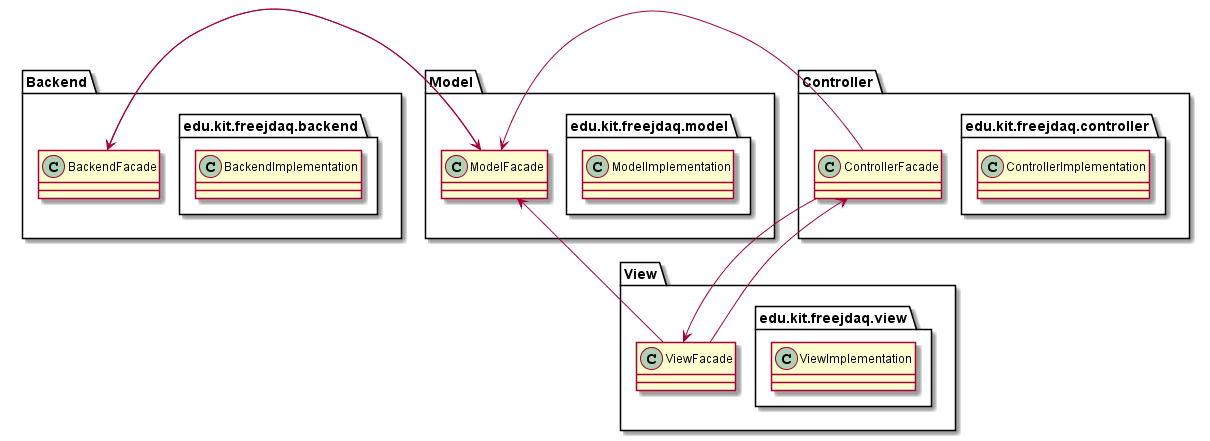
\includegraphics[width = 14cm]{Grafiken/Grober_Aufbau.png}
		\caption{Die grobe Struktur des Entwurfs}
		\label{Entwurf_Grob}
	\end{center}
\end{figure}


\clearpage
\section{Klassenbeschreibung}
Im folgenden sollen alle Klassen mit ihren Funktion beschrieben werden. Der Aufbau orientiert sich dabei an der in \ref{einleitung} aufgeführten Struktur.

\clearpage
\subsection{Backend}


\clearpage
\subsection{Model}

Das Modul Model stellt den Model-Teil des MVC-Entwurfsmusters da und ist für die Erstellung und Verwaltung der Datenstrukturen der Anwendung verantwortlich. Außerdem verarbeitet sie die Sensordaten so, dass diese in Graphen und Tabellen angezeigt werden können. Das Modul besteht dem Modulmanager, den Paketen Core, BuildingBlockBuilder, Sensor-, Transformation-, Representation- und ChannelLogic und diverser Fassaden.

\subsubsection{ModelManager}

\begin{figure}[htbp]
	\begin{center}
		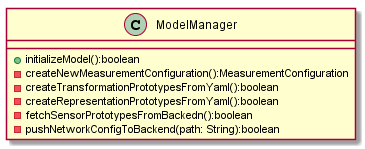
\includegraphics[width = 8cm]{Grafiken/ModelManager.png}
		\caption{Darstellung der Klasse ModelManager}
		\label{ModelManager}
	\end{center}
\end{figure}
Die Klasse ModelManager ist in Abbildung \ref{ModelManager} zu sehen. Sie hat die Aufgabe das Modul Model zu initialisieren. Dazu werden die folgenden sechs Methoden benutzt: 
\begin{itemize}

\item Die Methode \textit{initializeModel} initialisiert das Modul Model. Dabei nutzt sie vor allem die fünf anderen privaten Methoden.
\item Die private Methode \textit{createNewMeasurementConfiguration} erstellt eine neue leere Messkonfiguration für den Startbildschirm. 
\item Die private Methode \textit{createTransformationPrototypesFromYaml} lässt den Director des BuildingBlockBuilder-Pakets alle von der Anwendung angebotenen Transformationsprototypen erbauen und fügt diese dann dem BuildingBlockDirectory hinzu.
\item Die private Methode \textit{createRepresentationPrototypesFromYaml} lässt den Director des BuildingBlockBuilder-Pakets alle von der Anwendung angebotenen Darstellungsprototypen erbauen und fügt diese dann dem BuildingBlockDirectory hinzu.
\item Die private Methode \textit{fetchSensorPrototypesFromBackend} holt die Yaml-Dateien von dem Backend und lässt den Director des BuildingBlockBuilder-Pakets alle von der Anwendung angebotenen Sensorprototypen erbauen und fügt diese dann dem BuildingBlockDirectory hinzu.
\item Die private Methode \textit{pushNetworkConfigToBackend} liefert dem Backend die nötigen Netzwerkinformationen um mit dem RaspberryPi zu kommunizieren.

\end{itemize}



\subsubsection{Core}

\begin{figure}[htbp]
	\begin{center}
		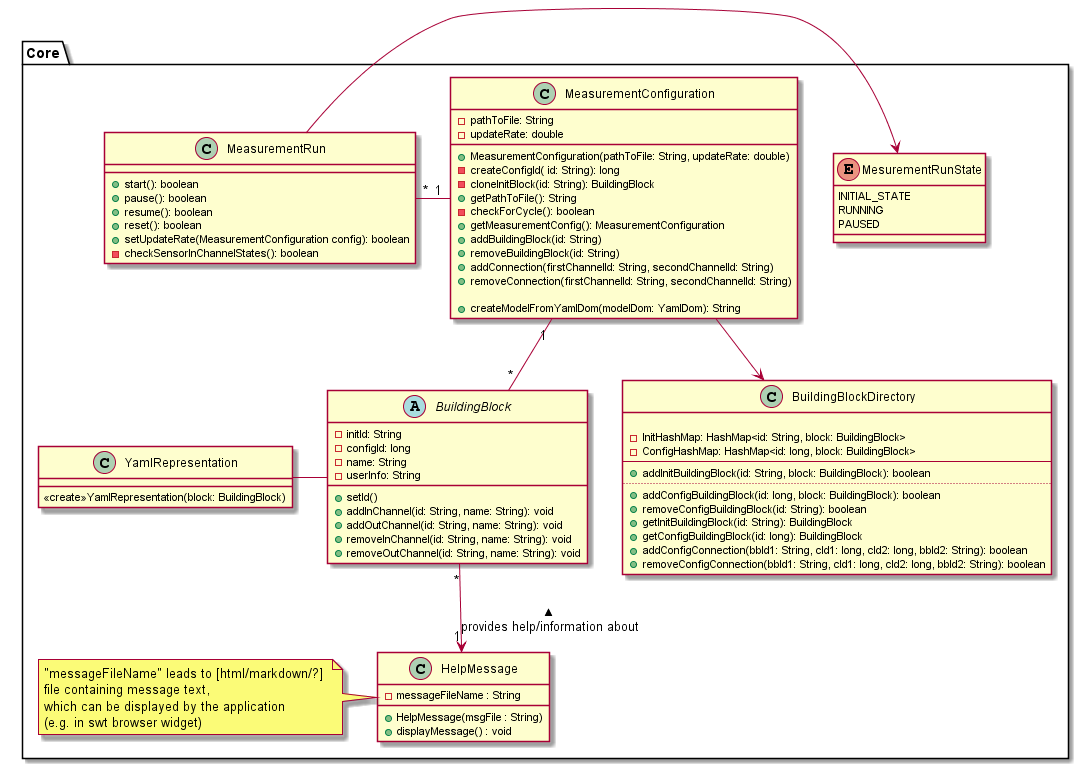
\includegraphics[width = 16cm]{Grafiken/ModelCore.png}
		\caption{Aufbau des Pakets Core}
		\label{ModelCore}
	\end{center}
\end{figure}

Die Struktur des Pakets Core ist in Abbildung \ref{ModelCore} zu sehen. Das Paket Core beinhaltet zentrale Klassen die für die Funktionalität des Models wichtig sind. 


\paragraph{BuildingBlockDirectory}

\begin{figure}[htbp]
	\begin{center}
		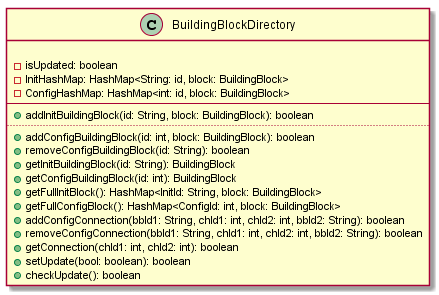
\includegraphics[width = 8cm]{Grafiken/BuildingBlockDirectory.png}
		\caption{Darstellung der Klasse BuildingBlockDirectory}
		\label{BuildingBlockDirectory}
	\end{center}
\end{figure}
Die Klasse BuildingBlockDirectory ist in Abbildung \ref{BuildingBlockDirectory} zu sehen.
Das erste Attribut der Klasse ist InitHashMap. Sie dient zur Speicherung einer HashMap, die von allen Bausteinen einer Messkonfiguration die initId speichert und zuordnet. Als zweites Attribut ist ConfigHashMap. Sie dient zur Speicherung einer HashMap, die von verfügbaren Prototypbausteinen die configId speichert und zuordnet. Das letzte Attribut isUpdated gibt an, ob d
Zur Verwaltung der Hashmaps sind folgende Methoden vorhanden:
\begin{itemize}

\item Die Methode \textit{addInitBuildingBlock} fügt der InitHashmap einen Bausteinprototypen hinzu.
\item Die Methode \textit{addConfigBuildingBlock} fügt der ConfigHashmap einen Baustein hinzu.
\item Die Methode \textit{removeConfigBuildingBlock} entfernt von der ConfigHashmap einen Baustein.
\item Die Methode \textit{getInitBuildingBlock} gewährt den Zugriff auf einen bestimmen Baustein der Messkonfiguration.
\item Die Methode \textit{getConfigBuildingBlock} gewährt den Zugriff auf einen bestimmen Bausteinprototypen.
\item Die Methode \textit{getFullInitBlock} gibt die Hashmap aller Bausteinprototypen als Rückgabewert zurück.
\item Die Methode \textit{getFullConfigBlock} gibt die Hashmap aller Bausteine der aktuellen Messkonfiguration als Rückgabewert zurück.

\item Die Methode \textit{addConfigConnection} fügt eine Verbindung zwischen zwei Bausteinen einer Messkonfiguration hinzu.
\item Die Methode \textit{removeConfigConnection} entfernt eine Verbindung zwischen zwei Bausteinen einer Messkonfiguration.
\item Die Methode \textit{getConnection} gibt an, ob zwei Kanäle verbunden sind.


\item Die Methode \textit{checkUpdate} prüft, ob ein der BuildingBlockDirectory aktuell ist.
\item Die Methode \textit{setUpdate} stellt den Status des BuildingBlockDirectory ein.
\end{itemize}

\paragraph{MeasurementConfiguration}
\begin{figure}[htbp]
	\begin{center}
		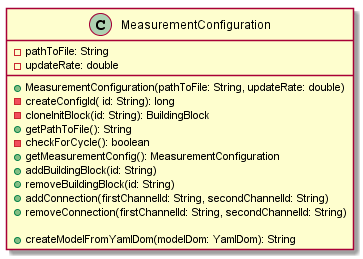
\includegraphics[width = 8cm]{Grafiken/MeasurementConfiguration.png}
		\caption{Darstellung der Klasse MeasurementConfiguration}
		\label{MeasurementConfiguration}
	\end{center}
\end{figure}
Die Klasse MeasurementConfiguration ist in Abbildung \ref{MeasurementConfiguration} zu sehen. Eine MeasurementConfiguration kann durch den Konstruktor MeasurementConfiguration erstellt werden. Sie hat dabei als erstes Attribut pathToFile einen Pfad zu dem Speicherort und als zweites Attribut updateRate. UpdateRate speichert den globalen Takt, mit der die Messkonfiguration einen Satz von Daten verarbeitet. Eine Instanz einer MeasurementConfiguration stellt im Model eine komplette Messkonfiguration dar. Diese wird durch die folgenden Methoden verwaltet:

\begin{itemize}

\item Die private Methode \textit{createConfigId} erstellt zu einem Bausteinprototypen eine ConfigId, um Instanzen des selben Bausteinprototypen unterscheiden zu können.
\item Die private Methode \textit{cloneInitBlock} erstellt eine Kopie eines Bausteinprototypen, gibt ihm eine neue ungenutzte configId und gibt diesen Block als Rückgabewert zurück.
\item Die Methode \textit{getPathToFile} liefert den Pfad zur Datei des Messkonfiguration.
\item Die private Methode \textit{checkForCycle} prüft die Messkonfiguration auf Zyklen.
\item Die Methode \textit{getMeasurementConfig} liefert eine Messkonfiguration.
\item Die Methode \textit{addBuildingBlock} fügt der Messkonfiguration einen Bausteinprototypen hinzu. Diese ist öffentlich verfügbar und greift auf die private Methode \textit{cloneInitBlock} zurück.
\item Die Methode \textit{removeBuildingBlock} entfernt einen Baustein von der Messkonfiguration, der durch die initId und die configId eindeutig bestimmt werden kann.
\item Die Methode \textit{addConnection} fügt eine Verbindung zwischen zwei Kanälen hinzu.
\item Die Methode \textit{removeConnection} entfernt eine Verbindung zwischen zwei Kanälen.
\item Die Methode \textit{createModelFromYamlDom} erstellt eine Messkonfiguration aus einer Datei.

\end{itemize}




\paragraph{MeasurementRun}
\begin{figure}[htbp]
	\begin{center}
		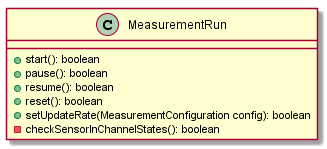
\includegraphics[width = 8cm]{Grafiken/MeasurementRun.png}
		\caption{Darstellung der Klasse MeasurementRun}
		\label{MeasurementRun}
	\end{center}
\end{figure}
Die Klasse MeasurementRun ist in Abbildung \ref{MeasurementRun} zu sehen. Ein MeasurementRun repräsentiert im Model einen Versuchslauf. Zu dessen Verwaltung gibt es folgende Methoden:


\begin{itemize}

\item Die Methode \textit{start} startet den Messlauf.
\item Die Methode \textit{pause} pausiert den Messlauf.
\item Die Methode \textit{resume} lässt den Messlauf fortfahren.
\item Die Methode \textit{reset} setzt die Fortschritte eines Messlaufs zurück und löscht alle bisher verarbeiteten Daten.
\item Die Methode \textit{setUpdateRate} überschreibt die Updaterate der zugehörigen Messkonfiguration. 
\item Die private Methode \textit{checkSensorInChannelStates} prüft den Status alles Eingangskanäle der Sensorbausteine. 

\end{itemize}


\subsubsection{BuildingBlock}
\begin{figure}[htbp]
	\begin{center}
		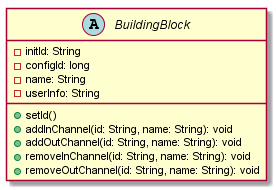
\includegraphics[width = 7cm]{Grafiken/BuildingBlock.png}
		\caption{Darstellung der Klasse BuildingBlock}
		\label{BuildingBlock}
	\end{center}
\end{figure}

Die abstrakte Klasse BuildingBlock ist in Abbildung \ref{BuildingBlock} zu sehen. Sie stellt im Model einen BuildingBlock dar und speichert die nötigen Daten als folgende Attribute:
\begin{itemize}

\item Das Attribut initId speichert als einen String eine eindeutige ID zur Unterscheidung von BuildingBlockPrototypen.
\item Das Attribut configId dient als eindeutige ID zur Unterscheidung von BuildingBlockInstanzen innerhalb einer Messkonfiguration, da auch mehrere BuildingBlocks eines Typs innerhalb einer Messkonfiguration auftreten können und unterschieden werden müssen.
\item Das Attribut name speichert den Namen einen BuildingBlocks als String dar. 
\end{itemize}
Ein BuildingBlock hat eine beliebige Menge an In- und OutChannels, deren Anzahl durch die folgenden Methoden verwaltet kann:

\begin{itemize}

\item Die Methode \textit{addInChannel} fügt dem BuildingBlock einen InChannel hinzu.
\item Die Methode \textit{removeInChannel} entfernt einen bestimmen InChannel von dem BuildingBlock.
\item Die Methode \textit{addOutChannel} fügt dem BuildingBlock einen OutChannel hinzu.
\item Die Methode \textit{removeOutChannel} entfernt einen bestimmen OutChannel von dem BuildingBlock.
\item Die Methode \textit{setConfigId} setzt die ConfigId des Bausteins, um ihn von anderen Instanzen des selben Bausteinprototyps unterscheiden zu können. 
\end{itemize}





\paragraph{YamlRepresentation}

Die Klasse YamlRepresentation erstellt aus einem Baustein eine Yaml-Datei. Dabei wird die Methode \textit{makeYamlRepresentation} benutzt.


\paragraph{HelpMessage}
Die Klasse HelpMessage enthält einen Konstruktor HelpMessage, der ein entsprechendes HelpMessage-Objekt erstellt.
Ein HelpMessage-Objekt speichert zu einem zugehörigen BuildingBlock einen Tooltip mit Informationen über den entsprechenden BuildingBlock. Die Verbindung zu der Datei, die die Informationen enthält, ist als Attribut messageFileName gespeichert. Die Methode
\textit{displayMessage} ermöglicht es, die Informationen anzuzeigen.



\subsubsection{MRunReaction}

\begin{figure}[htbp]
	\begin{center}
		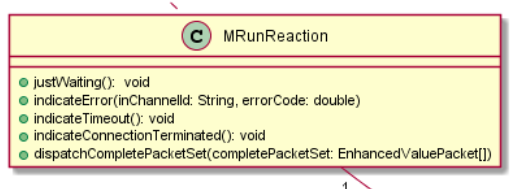
\includegraphics[width = 8cm]{Grafiken/MRunReaction.png}
		\caption{Darstellung der Klasse MRunReaction}
		\label{MRunReaction}
	\end{center}
\end{figure}

Die Klasse MRunReaction ist in Abbildung \ref{mRunReaction} zu sehen. Sie implementiert das Interface MRunForward, welches im Cache-Modul zu finden ist. MRunReaction dient als Verbindung zwischen Cache und Modul. Der Datenfluss vom Cache zu den Sensorbausteinen im Model wird durch die folgenden fünf Methoden verwaltet.
 
Die Methode \textit{justWaiting} signalisiert dem Modul, dass eine Verbindung besteht, aber kein Datenfluss stattfindet. Durch die Methode \textit{indicateError} dient dazu, dem Model das Auftreten eines Fehlers zu signalisieren. Dabei wird als Parameter ein Fehlercode und die ID des betroffenen Eingangschannels beigefügt. 
Durch die Methode \textit{timeOut} wird eine außerplanmäßige Unterbrechung einer Verbindung signalisiert. Durch die Methode \textit{connectionTerminated} wird hingegen das planmäßige Schließen einer Verbindung signalisiert. 
Die Methode \textit{dispatchCompletePacketSet} übergibt dem Model ein Set aus Datenpaketen, so dass jeder Eingangschannel jedes Sensors in der Messkonfiguration ein Packet erhält. Ein Datenpaket besteht hier aus Wert, Zielchannel und Zeitstempel.

\subsubsection{MRunInfo}

\begin{figure}[htbp]
	\begin{center}
		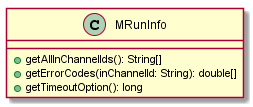
\includegraphics[width = 7cm]{Grafiken/MRunInfo.png}
		\caption{Darstellung der Klasse MRunInfo}
		\label{MRunInfo}
	\end{center}
\end{figure}



Die Klasse MRunInfo ist in Abbildung \ref{MRunInfo} zu sehen.
Sie implementiert das Interface MRunInfo vom Cache-Modul. Sie dient dazu, Informationen über den Datenfluss zu erhalten. Diese Informationen werden durch die drei folgenden Methoden erhalten:
 
\begin{itemize}

\item Die Methode \textit{getAllInChannelIds} übergibt dem Model alle Ids von aktiven Kanälen.
\item Die Methode \textit{getErrorCodes} übergibt dem Model die ErrorCodes der Kanäle. 
\item Die Methode \textit{getTimeoutOption} übergibt dem Model die Optionen für TimeOuts.


\end{itemize}


\subsubsection{FacadeViewModel}

\begin{figure}[htbp]
	\begin{center}
		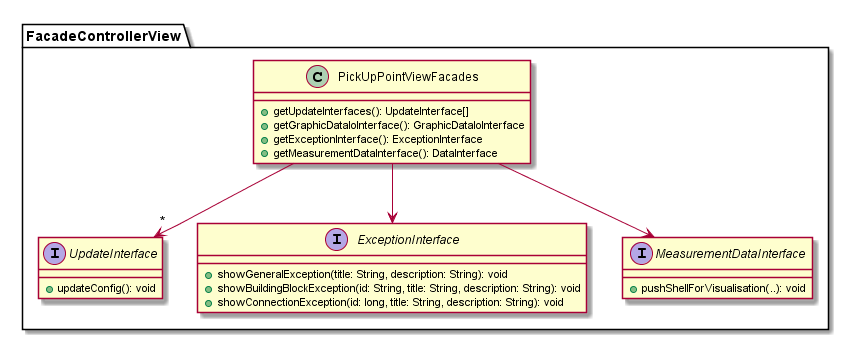
\includegraphics[width = 16cm]{Grafiken/FacadeViewModel.png}
		\caption{Aufbau des Pakets FacadeViewModel}
		\label{FacadeViewModel}
	\end{center}
\end{figure}

Die Struktur des Pakets FacadeViewModel ist in Abbildung \ref{FacadeViewModel} zu sehen. Das Paket FacadeViewModel stellt die Schnittstelle dar, die vom View angeboten und vom Model benutzt wird. Die Facade ist intern in drei Interfaces aufgeteilt um den nutzenden Klassen nur die benötigten Methoden zu übergeben. Die Interfaces sind über die PickUp-Klasse mit dem Modul verbunden.


\paragraph{PickUpPointViewFacades}
Die Klasse PickUpPointViewFacades stellt die Schnittstelle zwischen den Interfaces und dem Model dar und kapselt diese von einander. Durch ihre Methoden wird das entsprechende geforderte Interface zurückgegeben, dessen Methoden dann verwendet werden können.
\paragraph{MeasurementDataInterface}
Das Interface MeasurementDataInterface ermöglicht es dem Model, durch die Methode \textit{pushShellForVisualisation}, dem View einen XY-Graphen als Shell zu übergeben, der dann in der GUI dargestellt werden soll.
\paragraph{ExceptionInterface}
Das Interface ExceptionInterface ermöglicht es dem Model, dem View eine Exception zu übergeben. Durch die Methoden \textit{showGeneralException}, \textit{showBuildingBlockException} und \textit{showConnectionException} kann die Art der Exception konkretisiert werden.
\paragraph{UpdateInterface}
Das Interface UpdateInterface ermöglicht es dem Model der View durch die Methode \textit{updateConfig} die Veränderungen der Messkonfiguration zu signalisieren.




\subsubsection{SensorLogic}
\begin{figure}[htbp]
	\begin{center}
		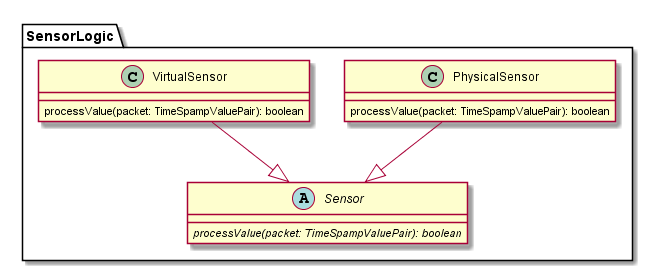
\includegraphics[width = 12cm]{Grafiken/SensorLogic.png}
		\caption{Aufbau des Pakets SensorLogic}
		\label{SensorLogic}
	\end{center}
\end{figure}

Die Struktur des Pakets SensorLogic ist in Abbildung \ref{SensorLogic} zu sehen. Das Paket speichert die Datenstrukturen von verschiedenen Arten von Sensorbausteinen. Dabei wird zwischen physischen Sensoren und virtuellen Sensoren unterschieden.



\paragraph{Sensor} Die abstrakte Klasse Sensor dient als Oberklasse aller Sensorbausteine im Model und gibt die Signatur der Methode \textit{processValue} als abstrakte Methode vor.


\paragraph{VirtualSensor}
Die Klasse VirtualSensor stellt einen Sensorblock dar, der Daten aus einen Datei liest. Dabei enthält die Datei Messwerte aus vergangenen Messläufen oder maschinell erzeugte Daten. Die Methode \textit{processValue} verarbeitet Daten, die über die Eingangskanäle eintreffen.

\paragraph{PhysicalSensor}
Die Klasse PhysicalSensor stellt einen Sensorblock dar, der Daten aus einem realen Sensor über das Backend erhält.  Die Methode \textit{processValue} verarbeitet Daten, die über die Eingangskanäle eintreffen.

\subsubsection{TransformationLogic}
\paragraph{Transformation}
\paragraph{Function}
\begin{figure}[htbp]
	\begin{center}
		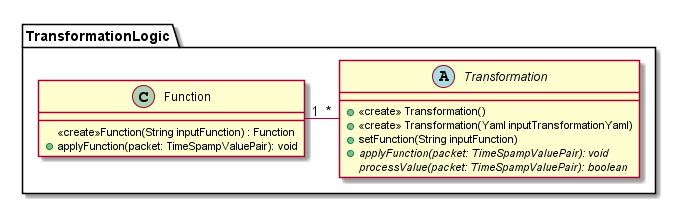
\includegraphics[width = 12cm]{Grafiken/TransformationLogic.png}
		\caption{Aufbau des Pakets TransformationLogic}
		\label{TransformationLogic}
	\end{center}
\end{figure}

Die Struktur des Pakets TransformationLogic ist in Abbildung \ref{TransformationLogic} zu sehen. Das Paket dient zur Repräsentation einer Transformation innerhalb des Models. Jeder Transformation hat genau eine Funktion, die sie auf die Daten aus Paketen anwendet.


\paragraph{Transformation}

Die Klasse Transformation hat zwei Konstruktoren. Ein Konstruktor erstellt eine Transformation aus einer Yaml-Datei. Der andere erstellt eine generische Transformation, die keine Yaml-Datei benötigt. Um Funktionalität der Transformation zu verwalten, werden folgende Methoden implementiert:

\begin{itemize}

\item Die Methode \textit{setFunction} setzt die Funktion, die die Transformation haben soll.
\item Die abstrakte Methode \textit{applyFunction} gibt die Signatur an. Die Methode wird dann in der Klasse Function implementiert.
\item Die Methode \textit{processValue} verarbeitet ein Paket, indem es die Funktion der Transformation auf den Wert des Pakets anwendet.


\end{itemize}

\paragraph{Function}

Die Klasse Function hat einen Konstruktor zu Erstellung einer Funktion aus einem String. Diese Funktion wird dann durch die Methode \textit{applyFunction} auf die Daten von Paketen angewendet.





\subsubsection{RepresentationLogic}
\begin{figure}[htbp]
	\begin{center}
		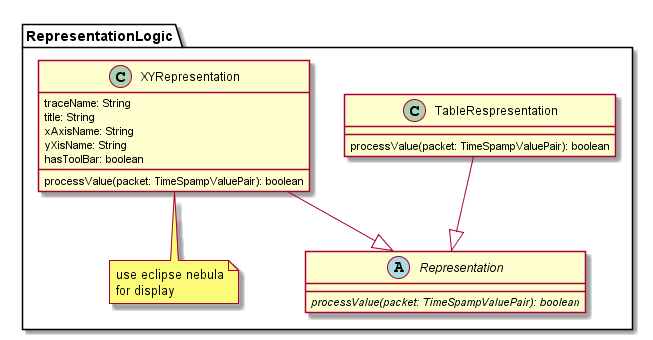
\includegraphics[width = 12cm]{Grafiken/RepresentationLogic.png}
		\caption{Aufbau des Pakets RepresentationLogic}
		\label{RepresentationLogic}
	\end{center}
\end{figure}
Die Struktur des Pakets RepresentationLogic ist in Abbildung \ref{RepresentationLogic} zu sehen. Das Paket dient zur Repräsentation einer Darstellung innerhalb des Models. Dabei wird zwischen Graphen und Tabellen unterschieden.

\paragraph{Representation}
Die abstrakte Klasse Sensor dient als Oberklasse aller Darstellungsbausteine im Model und gibt die Signatur der Methode \textit{processValue} als abstrakte Methode vor.

\paragraph{TableRepresentation}
Die Klasse TableRepresentation stellt im Model eine Darstellung von Daten durch eine Tabelle dar. Die Methode \textit{processValue} verarbeitet die eintreffenden Daten.
\paragraph{XYRepresentation}
Die Klasse XYRepresentation stellt im Model eine Darstellung von Daten durch einen Graph dar. Ein XYGraph die folgenden Attribute:

\begin{itemize}

\item Das Attribut traceName speichert den Namen des Traces.
\item Das Attribut title speichert den Titel des Graphen.
\item Das Attribut xAxisName speichtert den Namen der X-Achse.
\item Das Attribut yAXisName speichtert den Namen der Y-Achse.
\item Das Attribut hasToolBar gibt an, ob der Graph eine interaktive Toolbar anbietet.

\end{itemize}

Die Methode \textit{processValue} verarbeitet die eintreffenden Daten und erstellt mit Hilfe der externen Library Eclipse Nebula einen Graphen.

\subsubsection{ChannelLogic}

\begin{figure}[htbp]
	\begin{center}
		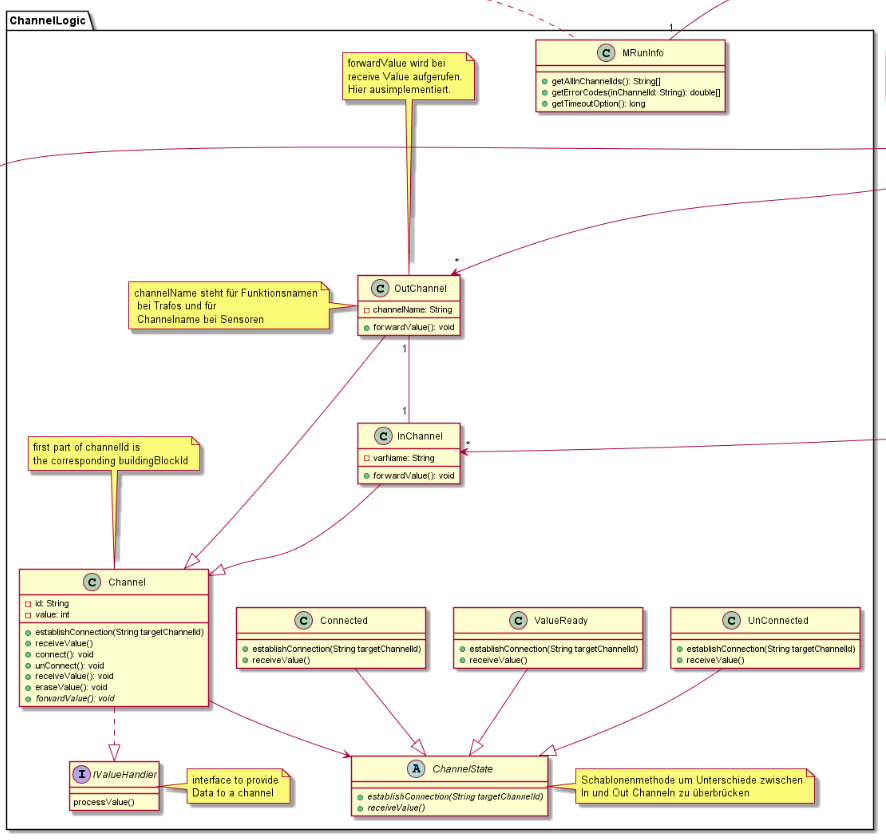
\includegraphics[width = 16cm]{Grafiken/ChannelLogic.png}
		\caption{Aufbau des Pakets ChannelLogic}
		\label{ChannelLogic}
	\end{center}
\end{figure}

Die Struktur des Pakets ChannelLogic ist in Abbildung \ref{ChannelLogic} zu sehen. Die Klasse repräsentiert die Datenstruktur eines Kanals. Dabei wird das Entwurfsmuster Zustand mit folgenden Rollen verwendet:
\begin{itemize}

\item Die Rolle der Clients wird durch die Klasse Channel erfüllt.
\item Die Rolle des Zustandes wird von der abstrakten Klasse ChannelState erfüllt.
\item Das Rolle des konkreten Zustandes wird durch die Klassen Connected, UnConnected und ValueReady erfüllt.

\end{itemize}

Das Entwurfsmuster ermöglicht es, die Anzahl der Zustände bei Bedarf zu erweitern.

\paragraph{Channel}
\begin{figure}[htbp]
	\begin{center}
		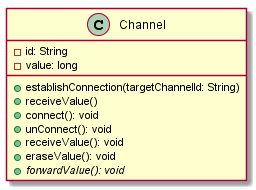
\includegraphics[width = 8cm]{Grafiken/Channel.png}
		\caption{Darstellung der Klasse Channel}
		\label{Channel}
	\end{center}
\end{figure}
Die Klasse Channel ist in Abbildung \ref{Channel} zu sehen.
Die Klasse Channel dient als Repräsentation eines Kanals im Model. Ein Kanal als Attribute eine eindeutige Id und einen Wert. Der Wert ist ein konkreter Wert eines Messlaufs und wird im Channel temporär zwischengespeichert.
Ein Kanal hat die Aufgabe Daten zu empfangen und wieder zu versenden. Außerdem dient er als Ausgangspunkt einer Verbindung unter verschiedenen Bausteinen. Um die Verbindung und den Datenfluss zu verwalten, hat ein Kanal folgende Methoden:

\begin{itemize}

\item Die Methode \textit{establishConnection} ermöglicht es dem Kanal eine Verbindung mit einem anderen Kanal einzugehen. Dabei ist nur eine Verbindung zwischen einem Eingangs- und einem Ausgangskanal möglich.
\item Die Methode \textit{receiveValue} ermöglicht es dem Kanal einen Wert zu empfangen.
\item Die Methode \textit{connect} wechselt den Zustand eines Kanals zu: vebundenen.
\item Die Methode \textit{unConnect} wechselt den Zustand eines Kanals zu: nicht vebundenen.
\item Die Methode \textit{eraseValue} löscht den Wert, der im Channel gespeichert ist.
\item Die abstrakte Methode \textit{forwardValue} dient dazu einen erhaltenen Wert weiter zu versenden. Die Implementierung der Methode ist in den Unterklassen zu finden.

\end{itemize}


\paragraph{InChannel}
Die Klasse InChannel ist eine Unterklasse von Channel und dient als Datenstruktur eines Eingangskanals im Model. Ein InChannel hat das zusätzliche Attribut varName, das den Namen des Eingangskanal speichert.
Die Methode \textit{forwardValue} wird hier implementiert.
\paragraph{OutChannel}
Die Klasse InChannel ist eine Unterklasse von Channel und dient als Datenstruktur eines Ausgangskanals im Model. Das zusätzliche Attribut channelName speichert den Namen den Ausgangskanals. Im Falle eines Ausgangskanal eines Sensorbausteins handelt es sich um Namen, der in der Yaml-Datei steht. Im Falle eines Ausgangskanals einer Transformation, wird hier der Name der Funktion gespeichert.
Die Methode \textit{forwardValue} wird hier implementiert.
\paragraph{ChannelState}
Die abstrakte Klasse ChannelState gibt als abstrakter Zustand die Signaturen der Methoden für der konkreten Zustände vor. Außerdem werden Unterschiede zwischen In- und OutChannel der Methoden \textit{establishConnection} und \textit{receiveValue} durch eine Schablonenmethode  überbrückt.

\paragraph{Connected}
Die Klasse Connected repräsentiert den verbundenen Zustand eines Kanals. 
\paragraph{UnConnected}
Die Klasse UnConnected repräsentiert den unverbundenen Zustand eines Kanals. 
\paragraph{ValueReady}
Die Klasse ValueReady repräsentiert einen "bin bereit"-Zustand des Kanal. Damit wird signalisiert, dass der Channel einen Wert erfolgreich empfangen hat und weiter versenden kann.

\subsubsection{BuildingBlockBuilder}
\begin{figure}[htbp]
	\begin{center}
		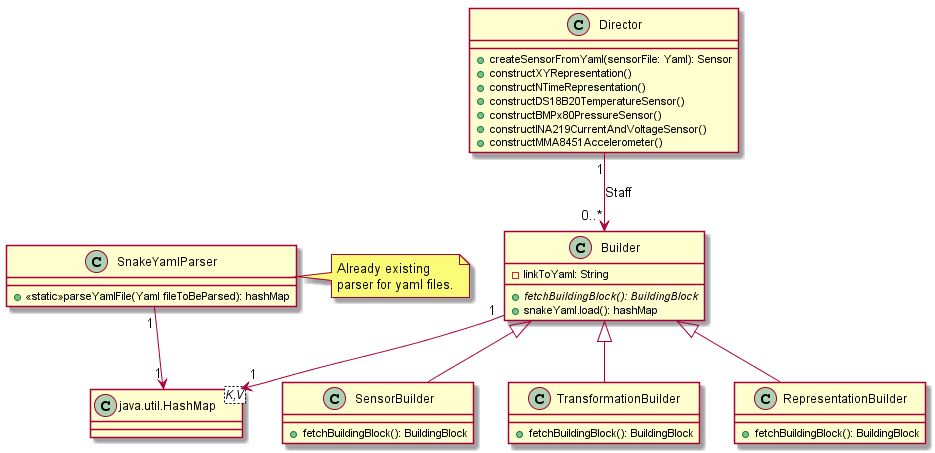
\includegraphics[width = 16cm]{Grafiken/BuildingBlockBuilder.png}
		\caption{Aufbau des Pakets BuildingBlockBuilder}
		\label{BuildingBlockBuilder}
	\end{center}
\end{figure}

Der Aufbau des Pakets BuildingBlockBuilder, zu sehen in Abbildung \ref{BuildingBlockBuilder}, setzt das Enwurfsmuster Erbauer um. Die Rollen sind dabei folgendermaßen umgesetzt:
\begin{itemize}

\item Die Klasse \textit{Director} erfüllt die Rolle des \textit{Direktors}.
\item Die Klasse \textit{Builder} erfüllt die Rolle eines \textit{Erbauers}.
\item Die Klassen \textit{SensorBuilder},\textit{TransformationBuilder}, \textit{RepresentationBuilder},
\textit{VirtualSensorBuilder},\textit{PhysicalSensorBuilder},\textit{XYRepresentationBuilder} und \textit{TableRepresentationBuilder}  erfüllen die Rolle der \textit{konkreten Erbauer}.
\item Die Rollen der \textit{Produkte} werden in den Paketen \hyperlink{SensorLogic}{SensorLogic}, \hyperlink{TransformationLogic}{TransformationLogic} und \hyperlink{RepresentationLogic}{RepresentationLogic} als entsprechende Bausteine erfüllt.

\end{itemize} 
Hier wurde bewusst das Erbauer Entwurfsmuster ausgewählt, da es leicht erweitern lässt, in dem man eine Methode im Director und einen konkreten Erbauer hinzufügt. Wir haben uns gegen die abstrakte Fabrik entschieden, da sich diese schwerer erweitern lässt.

\paragraph{Director}
\begin{figure}[htbp]
	\begin{center}
		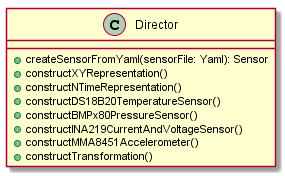
\includegraphics[width = 7cm]{Grafiken/Director.png}
		\caption{Darstellung der Klasse Director}
		\label{Director}
	\end{center}
\end{figure}
Die Klasse Director ist in Abbildung \ref{Director} zu sehen. Sie bietet eine Reihe an \textit{construct...} Methoden an, mit denen konkrete BuildingBlocks erstellt werden können. Der resultierende BuildingBlock wird dann in einer HashMap im BuildingBlockDirectory abgelegt. Dabei kann die Auswahl an Methoden durch neue Methoden erweitert werden, um neue Arten von Blöcken erbauen zu können. Dabei muss auch jeweils ein neuer konkreter Erbauer implementiert werden. In erster Linie hat der Director die Aufgabe, beim Start der Anwendung die angebotenen Prototypen zu erstellen und im BuildingBlockDirectory zu speichern. 

\paragraph{Builder}
Die Klasse Builder ist die Oberklasse aller konkreten Builder. Sie hat als Attribut eine Verbindung zu einer Yaml-Datei. Mit Hilfe dieser Yaml-Datei kann ein entsprechender BuildingBlock erstellt werden. Die Yaml-Datei wird durch die Methode \textit{snakeYaml.load} geladen, welche durch das externe Paket SnakeYamlParser angeboten wird. Die abstrakte Methode \textit{fetchBuildingBlock} gibt die Signatur für die konkreten Erbauer vor. In den konkreten Erbauern kann der Director durch diese Methode einen entsprechenden BuildingBlock anfordern und als Rückgabewert erhalten, sobald er erbaut wurde. 

\paragraph{SensorBuilder}
Die Klasse erstellt als konkreter Erbauer durch Aufrufen der Methode \textit{fetchBuildingBlock} aus einer Yaml-Datei einen TransformationsBlock und gibt ihn als Rückgabewert zurück. Die Verbindung zu der entsprechenden Yaml-Datei wird als Attribut von der Oberklasse Builder geerbt.


\paragraph{VirtualSensorBuilder}
Die Klasse erstellt als konkreter Erbauer durch Aufrufen der Methode \textit{fetchBuildingBlock} aus einer Yaml-Datei einen VirtualsensorBlock und gibt ihn als Rückgabewert zurück. Die Verbindung zu der entsprechenden Yaml-Datei ist als geerbtes Attribut vorhanden.
\paragraph{PhysicalSensorBuilder}
Die Klasse erstellt als konkreter Erbauer durch Aufrufen der Methode \textit{fetchBuildingBlock} aus einer Yaml-Datei einen PhysicalSensorBlock und gibt ihn als Rückgabewert zurück. Die Verbindung zu der entsprechenden Yaml-Datei ist als geerbtes Attribut vorhanden. Der PhysicalSensorBuilder fügt dem Sensorblock durch die Methode \textit{addSensorProducerName} zusätzlich noch den Werknamen des Sensors hinzu.
\paragraph{TransformationBuilder}
Die Klasse erstellt als konkreter Erbauer durch Aufrufen der Methode \textit{fetchBuildingBlock} aus einer Yaml-Datei einen TransformationsBlock und gibt ihn als Rückgabewert zurück. Die Verbindung zu der entsprechenden Yaml-Datei wird als Attribut von der Oberklasse Builder geerbt.

\paragraph{RepresenstationBuilder}
Die Klasse erstellt als konkreter Erbauer durch Aufrufen der Methode \textit{fetchBuildingBlock} aus einer Yaml-Datei einen RepresentationBlock und gibt ihn als Rückgabewert zurück. Die Verbindung zu der entsprechenden Yaml-Datei wird als Attribut von der Oberklasse Builder geerbt.
\paragraph{TableRepresenstationBuilder}
Die Klasse erstellt als konkreter Erbauer durch Aufrufen der Methode \textit{fetchBuildingBlock} aus einer Yaml-Datei einen TableRepresentationBlock und gibt ihn als Rückgabewert zurück. Die Verbindung zu der entsprechenden Yaml-Datei wird als Attribut von der Oberklasse Builder geerbt.
\paragraph{XYRepresenstationBuilder}
Die Klasse erstellt als konkreter Erbauer durch Aufrufen der Methode \textit{fetchBuildingBlock} aus einer Yaml-Datei einen XYRepresentationBlock und gibt ihn als Rückgabewert zurück. Die Verbindung zu der entsprechenden Yaml-Datei wird als Attribut von der Oberklasse Builder geerbt.
\paragraph{java.util.HashMap}
Die Klasse repräsentiert die Struktur des Datentyps, der durch die Klasse SnakeYamlParser verwendet wird.
\paragraph{SnakeYamlParser}
Diese Klasse stellt ein externes Paket dar, welches den SnakeYamlParser implementiert.

\clearpage
\subsection{Controller}

\begin{figure}[htbp]
	\begin{center}
		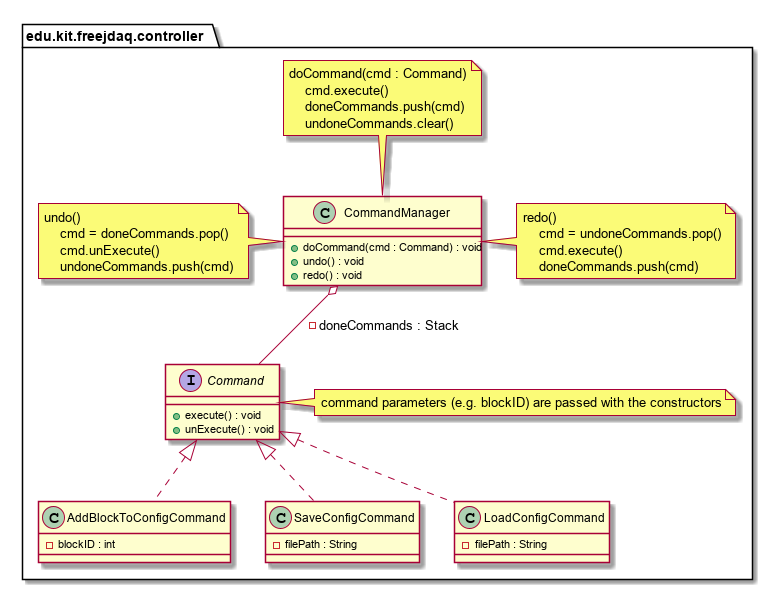
\includegraphics[width = 14cm]{Grafiken/Controller_Struktur.png}
		\caption{Die Struktur des Controllers (Ausschnitt)}
		\label{Controller_Struktur}
	\end{center}
\end{figure}

Der Aufbau des Controllers setzt das Entwurfsmuster \textit{Kommando} (\textit{Command}) um. Die Rollen sind dabei folgendermaßen:

\begin{itemize}

\item Die Klasse \textit{CommandManager} erfüllt die Rolle des \textit{Aufrufers} (\textit{Invoker}).
\item Die Schnittstelle \textit{Command} erfüllt die Rolle eines \textit{Befehls} im abstrakten Sinne.
\item Die Klassen, welche \textit{Command} implementieren, erfüllen die Rolle der \textit{konkreten Befehle}.
\item Die Rolle des (bzw. der) \textit{Klienten} wird durch die Klassen \textit{ButtonAction}, \textit{BlockAction}, bzw. \textit{ConnectionAction} erfüllt. Diese bilden die Schnittstelle, über welche das \textit{View}-Modul auf den Controller zugreift.
\item Die Rolle der \textit{Empfänger} wird durch die Schnittstelle(n) zum \textit{Model}-Modul erfüllt.

\end{itemize}

\subsubsection{CommandManager}

\begin{figure}[htbp]
	\begin{center}
		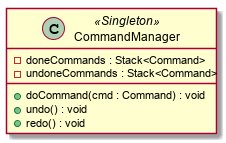
\includegraphics[width = 6cm]{Grafiken/CommandManager.png}
		\caption{Die Klasse CommandManager}
		\label{CommandManager}
	\end{center}
\end{figure}

Die Klasse CommandManager hat die Funktion, die Ausführung konkreter Befehle zu veranlassen. Der CommandManager ist als \textit{Singleton} definiert um sicherzustellen, dass von allen Klienten auf dieselbe Instanz zugegriffen wird.

Anhand eines \textit{Undo-} und eines \textit{Redo-Stacks} bietet der CommandManager außerdem die Möglichkeit an, bereits ausgeführte Befehle rückgängig zu machen (bzw. rückgängig gemachte Aktionen wiederherzustellen). Nicht alle Befehle können rückgängig gemacht werden.

Die Verwendung des Command-Musters ermöglicht zudem Erweiterungsmöglichkeiten wie beispielsweise eine Warteschlange für Befehle. Falls nötig können derartige Erweiterungen umgesetzt werden, ohne Programmcode außerhalb des Entwurfsmusters verändern zu müssen.

\subsubsection{Command bzw. konkrete Befehle}

Die Schnittstelle Command und die konkreten Klassen, welche die Schnittstelle implementieren, sind die Befehle des Controllers. Jeder konkrete Befehl kapselt eine genau definierte Funktionalität. Weitere Befehle können problemlos hinzugefügt werden, ohne bestehende Klassen verändern zu müssen.

Beim konstruieren eines Befehlobjektes können gegebenenfalls Parameter übergeben werden, beispielsweise eine eindeutige \textit{Block-ID} für Bausteine. Durch Aufrufen der \textit{execute()}-Methode wird der jeweilige Befehl ausgeführt.

Bestimmte Befehle können durch \textit{unExecute()} rückgängig gemacht werden. In diesen Fällen wird von \textit{isUndoable()} immer \textit{true} zurückgegeben.

Andere Befehle können nicht rückgängig gemacht werden. Dann ist die Methode \textit{unExecute()} leer und \textit{isUndoable()} gibt \textit{false} zurück.

\begin{figure}[htbp]
	\begin{center}
		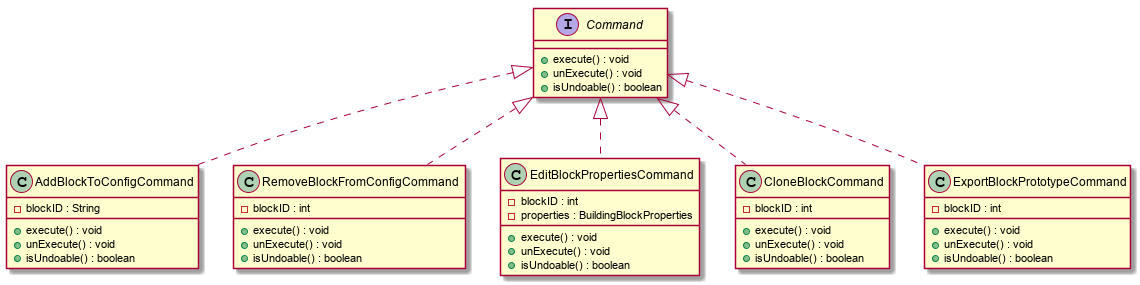
\includegraphics[width = 14cm]{Grafiken/Commands1.png}
		\caption{Baustein-Befehle}
		\label{Commands1}
	\end{center}
\end{figure}

\paragraph{AddBlockToConfigCommand}

Dieser Befehl fügt einen gegebenen Baustein zum Konfigurationsfeld hinzu und kann rückgängig gemacht werden.

\paragraph{RemoveBlockFromConfigCommand}

Dieser Befehl entfernt einen Baustein aus dem Konfigurationsfeld und kann rückgängig gemacht werden.

\paragraph{EditBlockPropertiesCommand}

Dieser Befehl verändert die Eigenschaften eines Bausteins.

\paragraph{CloneBlockCommand}

Dieser Befehl klont einen bestehenden Bausteinprototyp.

\paragraph{ExportBlockPrototypeCommand}

Dieser Befehl exportiert einen Bausteinprototypen als Datei.

\begin{figure}[htbp]
	\begin{center}
		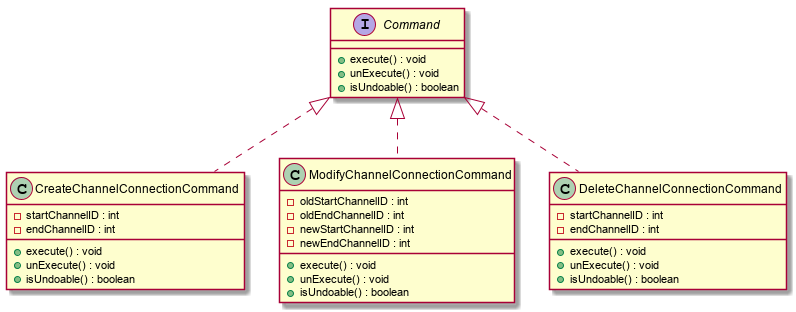
\includegraphics[width = 10cm]{Grafiken/Commands2.png}
		\caption{Verbindungs-Befehle}
		\label{Commands2}
	\end{center}
\end{figure}

\paragraph{CreateChannelConnectionCommand}

Dieser Befehl erstellt eine Verbindung zwischen zwei gegebenen Kanälen (welche wiederum zu Bausteinen gehören) und kann rückgängig gemacht werden.

\paragraph{ModifyChannelConnectionCommand}

Dieser Befehl verändert Start- und/oder Endpunkt einer Verbindung zwischen zwei Kanälen und kann rückgängig gemacht werden.

\paragraph{DeleteChannelConnectionCommand}

Dieser Befehl löscht eine Verbindung zwischen zwei Kanälen und kann rückgängig gemacht werden.

\begin{figure}[htbp]
	\begin{center}
		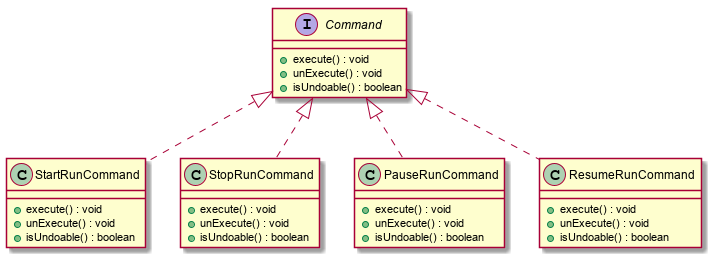
\includegraphics[width = 12cm]{Grafiken/Commands3.png}
		\caption{Messlauf-Befehle}
		\label{Commands3}
	\end{center}
\end{figure}

\paragraph{StartRunCommand}

Dieser Befehl startet einen Messlauf.

\paragraph{StopRunCommand}

Dieser Befehl beendet einen aktiven Messlauf.

\paragraph{PauseRunCommand}

Dieser Befehl pausiert einen aktiven Messlauf.

\paragraph{ResumeRunCommand}

Dieser Befehl setzt einen pausierten Messlauf fort.

\begin{figure}[htbp]
	\begin{center}
		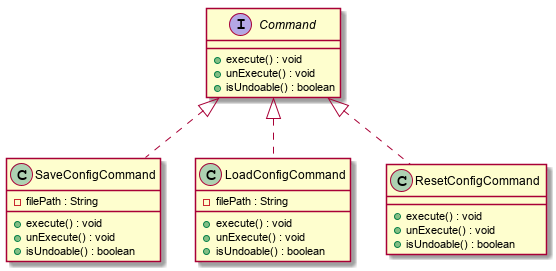
\includegraphics[width = 10cm]{Grafiken/Commands4.png}
		\caption{Messkonfigurations-Befehle}
		\label{Commands4}
	\end{center}
\end{figure}

\paragraph{SaveConfigCommand}

Dieser Befehl speichert die aktuelle Messkonfiguration an einem übergebenen Dateipfad.

\paragraph{LoadConfigCommand}

Dieser Befehl lädt eine Messkonfiguration von einem angegebenen Pfad.

\paragraph{ResetConfigCommand}

Dieser Befehl entfernt alle Elemente aus dem Konfigurationsfeld. (Verwendung optional.)

\subsubsection{Verbindung zum View}

\begin{figure}[htbp]
	\begin{center}
		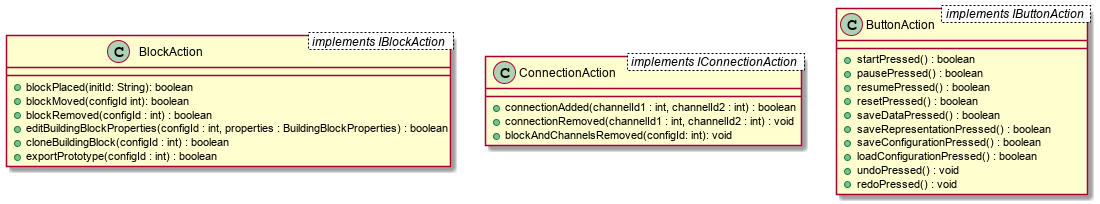
\includegraphics[width = 14cm]{Grafiken/View_Controller_Interface.png}
		\caption{Schnittstellenimplementierung View zu Controller}
		\label{View_Controller_Interface}
	\end{center}
\end{figure}

Durch das View-Modul werden mehrere Schnittstellen definiert, anhand derer die View-Klassen die Ausführung von Befehlen veranlassen können. (Abschnitt 2.4.9)

\paragraph{BlockAction} Die Klasse BlockAction implementiert die Schnittstelle IBlockAction des Views.

\paragraph{ButtonAction} Die Klasse ButtonAction implementiert die Schnittstelle IButtonAction des Views.

\paragraph{ConnectionAction} Die Klasse ConnectionAction implementiert die Schnittstelle IConnectionAction des Views.

\subsubsection{Verbindung zum Model}

\begin{figure}[htbp]
	\begin{center}
		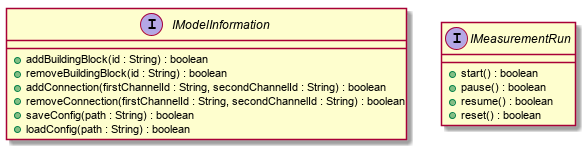
\includegraphics[width = 14cm]{Grafiken/Controller_Model_Interface.png}
		\caption{Schnittstelle Controller zu Model}
		\label{Controller_Model_Interface}
	\end{center}
\end{figure}

Es werden Schnittstellen vorgegeben, die durch das Model-Modul implementiert werden. Ihre Methoden erlauben es den Klassen des Controllers, gezielt auf Funktionalität des Models zuzugreifen.

\paragraph{IModelInformation}

Diese Schnittstelle stellt Methoden zur Verfügung, anhand derer die Messkonfiguration und darin enthaltene Bausteine verändert werden können.

\paragraph{IMeasurementRun}

Diese Schnittstelle stellt Methoden zur Verfügung, anhand derer ein Messlauf gestartet, beendet, angehalten und fortgeführt werden kann.

\clearpage
\subsection{View}
Das Paket View, stellt gemäß des MVC- Entwurfmusters die Darstellungen des Modells dar und realisiert Benutzerinteraktionen auf der graphischen Benutzeroberfläche. 

\subsubsection{MainWindow} 

\begin{figure}[htbp]
	\begin{center}
		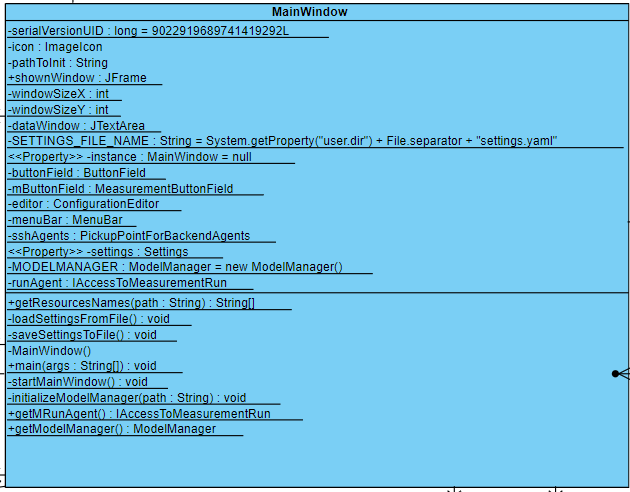
\includegraphics[width = 5cm]{Grafiken/View/MainWindow.png}
		\caption{Die Klasse MainWindow}
		\label{MainWindow}
	\end{center}
\end{figure}

Die Klasse MainWindow, zu sehen in Abbildung \ref{MainWindow}, stellt den Rahmen der Benutzeroberfläche dar. Alle Restlichen graphischen Oberflächen werden durch das MainWindow instanziert. Dazu gehört das Konfigurationsfeld, Buttonmenü, Konfigurationsbausteinmenü, Hilfe , Optionen und Fehlerfenster. 
Da MainWindow, dass Entwurfsmuster Singleton verwendet, kann die Anwendung nur ein MainWindow besitzen soll.
Bei Schließen des MainWindow wird ebenso die gesamte Anwendung beendet.

\newpage

\subsubsection{Menues}

\begin{figure}[htbp]
	\begin{center}
		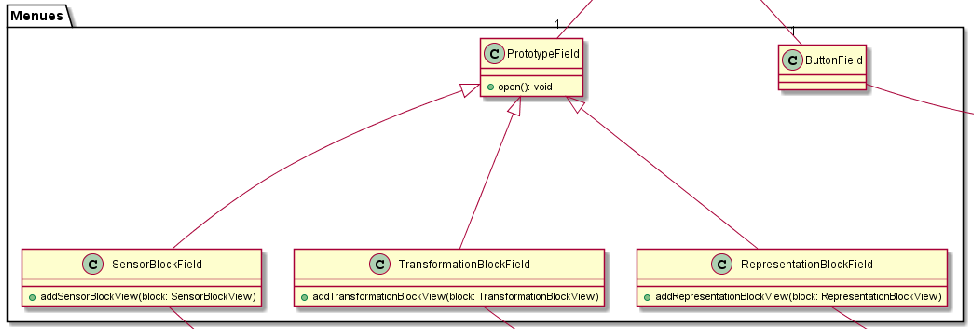
\includegraphics[width = 14cm]{Grafiken/View/MenuesNamespace.png}
		\caption{Aufbau des Menü-Paket}
		\label{Menues}
	\end{center}
\end{figure}

Menüs bieten dem Benutzer eine übersichtliche visuelle Zusammenfassung der Darstellungen der konkreten Bausteine und Knöpfe. 


\paragraph{PrototypeField}
Die Klasse PrototypeField ist die Über-Klasse zu SensorBlockField, TransformationBlockField und RepresentationBlockField. 
Sie stellt die Menüfläche dar, in welcher vordefinierte Konfigurationsbausteine je nach Kategorie dargestellt werden und der Benutzer sie mit dem Mauszeiger in das Konfigurationsfeld ziehen und damit positionieren kann. Diese vordefinierten Bausteine werden über das Backend eingelesen und werden über das Model im Directory zur Verwendung auf der Benutzeroberfläche bereitgestellt.

\paragraph{FieldHandler}
Das Interface FieldHandler nimmt Benutzereingaben entgegen, in diesem Fall werden das Öffnen der Menüflächen registiert und an das Feld weitergeleitet.

\paragraph{SensorBlockField}
Die Klasse SensorBlockField stellt die Menüfläche dar, in welcher alle Sensorbausteine angezeigt werden.

\paragraph{TransformationBlockField}
Die Klasse TransformationBlockField stellt die Menüfläche dar, in welcher alle Transformationsbausteine angezeigt werden.

\paragraph{RepresentationBlockField}
Die Klasse RepresentationBlockField stellt die Menüfläche dar, in welcher alle Representationsbausteine angezeigt werden.

\paragraph{ButtonField}
Die Klasse ButtonField stellt die Menüfläche dar, in welcher alle konkreten Knöpfe platziert sind und diese für den Benutzer verwendbar sind.

\subsubsection{Configuration}


\paragraph{ConfigurationField}

\begin{figure}[htbp]
	\begin{center}
		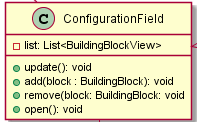
\includegraphics[width = 6cm]{Grafiken/View/ConfigurationField.png}
		\caption{Aufbau des Konfigurationsfeld}
		\label{Konfigurationsfeld}
	\end{center}
\end{figure}

Die Klasse KonfigurationField, zu sehen in Abbildung \ref{Konfigurationsfeld} stellt das Konfigurationsfeld dar, in welchem der Benutzer eine Messkonfiguration aufbauen kann.
Konfigurationsbausteine, welche der Benutzer in das Konfigurationsfeld platziert werden in einer Liste gespeichert. 
Konfigurationsbausteine, welche der Benutzer aus dem Konfigurationsfeld entfernt, werden aus der Liste gelöscht
Beim Platzieren der Konfigurationsbausteine in das Konfigurationsfeld wird dem Konfigurationsbaustein eine eindeutige Position zugeteilt, welche in Form von einer x-Koordinate und einer y-Koordinate dargestellt wird.
Die Liste der Bausteine kann ebenfalls von außerhalb ausgelesen oder gesetzt werden, falls z.B die Anordnung der Bausteine und Verbindungen gespeichert oder gesetzt werden soll.

\newpage

\begin{figure}[htbp]
	\begin{center}
		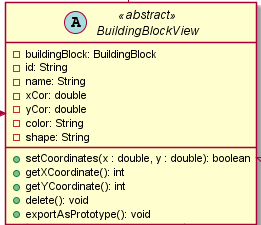
\includegraphics[width = 7cm]{Grafiken/View/BuildingBlockView.png}
		\caption{Aufbau des BuildingBlockView}
		\label{BuildingBlockView}
	\end{center}
\end{figure}

\paragraph{BuildingBlockView}


Die Klasse BuildingBlockView ist in Abbildung \ref{BuildingBlockView} zu sehen. Sie stellt die Überklasse der Darstellungen der Konfigurationsbausteine.
Bausteine werden über das Directory erzeugt, indem zu jedem im Directory gespeicherten Baustein eine Darstellung dieses Bausteins erzeugt wird. Name und InitId bleiben bei Erzeugung des Bausteins gleich, jedoch wird der Baustein, um die visuellen Komponenten Koordinaten, Farbe, Form und Größe erweitert.
Konfigurationsbausteine besitzen eine eindeutige Initialisierungs-ID, darunter versteht man die ID, welche der Baustein beim Erstellen durch das Model bekommt. Jede konkrete Instanz dieses Baustein besitzt diese Initialsierungs-ID (InitId). Wenn ein Baustein mehrfach durch den Benutzer in das Konfigurationsfeld gezogen wird, könnte dies dazu führen, dass diese Initialisierungs-ID nicht mehr eindeutig für diesen Baustein wäre. Deswegen besitzt jeder im Konfigurationsfeld platzierte Baustein eine Konfigurations-ID. Diese ID ist eindeutig für diesen Baustein und somit ist dieser Baustein unterscheidbar von weiteren Bausteinen gleichem Prototyps. Ebenfalls besitzt ein Baustein einen Namen und falls sie im Konfigurationsfeld platziert werden ihre Position anhand der Koordinaten x und y. Form, Farbe und Größe sind ebenfalls festgelegt.  
Bausteine werden über das Directory erzeugt, indem zu jedem im Directory gespeicherten Baustein eine Darstellung dieses Bausteins erzeugt wird. Name und InitId bleiben bei Erzeugung des Bausteins gleich, jedoch wird der Baustein, um die visuellen Komponenten Koordinaten, Farbe, Form erweitert.


\begin{figure}[htbp]
	\begin{center}
		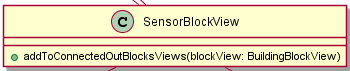
\includegraphics[width = 7cm]{Grafiken/View/SensorBlockView.png}
		\caption{Aufbau des SensorBlockView}
		\label{Entwurf_Grob}
	\end{center}
\end{figure}

\paragraph{SensorBlockView}

Die Klasse SensorBlockView stellt einen Sensorbaustein dar. 
Sensorbausteine, welche in dem Konfigurationsfeld platziert werden, können mit anderen Bausteinen verbunden werden, was im Messlauf einen Datenfluss über die verbundenen Bausteine erlaubt. Sensorbausteine besitzen, im Gegensatz zu anderen Konfigurationsbausteinen nur Datenausgänge, über welche sie verbunden werden können, da Sensoren, gemäß physikalischer 
Repräsentation nur Datenausgänge besitzen.

\paragraph{TransformationBlockView}

\begin{figure}[htbp]
	\begin{center}
		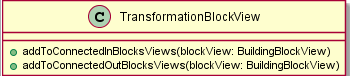
\includegraphics[width = 7cm]{Grafiken/View/TransformationBlockView.png}
		\caption{Aufbau des TransformationBlockView}
		\label{Entwurf_Grob}
	\end{center}
\end{figure}

Die Klasse TransformationBlockView ist die visuelle Darstellung einer Transformation dar. Transformationsbausteine besitzen eine vordefinierte Funktion, welche die Messdaten nach der Funktion transformiert. Transformationbausteinen besitzen Eingänge, welche Daten von Sensorenbausteinen oder anderen Transformationenbausteinen empfangen können. Ausgänge der Transformationsbausteine können nur an weitere Transformationsbausteine oder Darstellungsbausteine angebunden werden, um einen sinnvollen Datenfluss zu ermöglichen. 

\paragraph{RepresentationBlockView} 

\begin{figure}[htbp]
	\begin{center}
		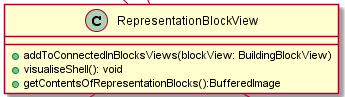
\includegraphics[width = 9cm]{Grafiken/View/RepresentationBlockView.png}
		\caption{Aufbau des RepresentationBlockView}
		\label{Entwurf_Grob}
	\end{center}
\end{figure}

Die Klasse RepresentationBlockView stellt einen Darstellungbaustein dar, dieser bestimmt, wie die Messdaten visualisiert werden. Dafür bekommt der Repräsentationsbaustein die visuelle Darstellung in dem Darstellungsgerüst (z.B: Graph, Tabelle) mit den dargestellten Messdaten.
Zur Speicherung der visuellen Darstellung der Daten muss ein Bild erstellt werden, welches zum Speichern weiter geleitet wird.
Darstellungsbausteine besitzen nur Eingänge, da visualisierte Messdaten nicht mehr verarbeitet werden. 

\clearpage

\begin{figure}[htbp]
	\begin{center}
		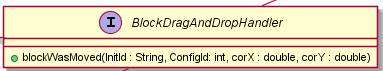
\includegraphics[width = 9cm]{Grafiken/View/BlockDragAndDropHandler.png}
		\caption{Aufbau des BlockDragAndDropHandler}
		\label{BlockDragAndDropHandler}
	\end{center}
\end{figure}

\paragraph{BlockDragAndDropHandler}

Über das Interface BlockDragAndDropHandler, welches in Abbildung \ref{BlockDragAndDropHandler} zu sehen ist, wird der Anwendung mitgeteilt, dass ein Konfigurationsbaustein durch Drag-and-Drop in der GUI bewegt wurde. Es wird übergeben, um welchen eindeutigen Konfigurationsbaustein es sich handelt, indem bei Konfigurationsbausteinen, welche zuvor nicht im Konfigurationsfeld platziert die Initialisierungs-ID übergeben wird. Bei Konfigurationsbausteinen, welche bereits im Konfigurationsfeld liegen und nicht mehr durch die Initialisierungs-ID eindeutig unterscheidbar sind, wird die Konfigurations-ID übergeben. Ebenfalls wird die Position auf welche der Konfigurationsbaustein gesetzt wurde durch die x- und y- Koordinaten mitübergeben.

\begin{figure}[htbp]
	\begin{center}
		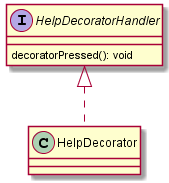
\includegraphics[width = 5cm]{Grafiken/View/HelpDecorator.png}
		\caption{Klasse HelpDecorator mit Interface HelpDecoratorHandler}
		\label{Help}
	\end{center}
\end{figure}

\paragraph{HelpDecorator}

Jeder Konfigurationsbaustein besitzt eine kurze Beschreibung seiner Art und Funktionalität. Diese Beschreibung wird über das Fenster der Klasse HelpDecorater dem Benutzer dargestellt. Die Abbildung der Klasse ist in Abbildung \ref{Help} zu sehen.

\paragraph{HelpDecoratorHandler}

Das Interface HelpDecoraterHandler, zu sehen in Abbildung \ref{Help} wird von der Klasse HelpDecorater implementiert und registriert wenn der Benutzer den HelpDecorater öffnen will, in dem er darauf drückt.

\begin{figure}[htbp]
	\begin{center}
		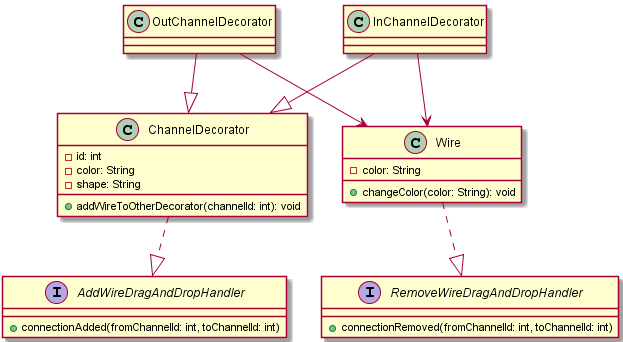
\includegraphics[width = 13cm]{Grafiken/View/ChannelDecorator.png}
		\caption{Aufbau der ChannelDecorator-Logik}
		\label{ChannelDecorator}
	\end{center}
\end{figure}

\paragraph{ChannelDecorator}

Die Klasse ChannelDecorater stellt die Überklasse zu den Klassen InChannelDecorator und OutChannelDecorator dar. 
Ein ChannelDecorater ist ein Objekt, welches durch Konfigurationsbausteine instanziiert werden. Ein ChannelDecorater stellt die Schnittstelle zu anderen ChannelDecorater dar, um zwei Bausteine miteinander zu verbinden. Dies geschiet durch die Methode addWireToOtherDecorator. Um diese ChannelDecorater eindeutig unterscheiden zu können besitzten diese eine eindeutige ID. Zur visuellen Repräsentation der Ein- und Ausgänge besitzen diese eine Farbe und Form.

\paragraph{InChannelDecorator}

Die Klasse InChannelDecorator erbt von der Klasse ChannelDecorater und stellt einen Kanaleingang eines Konfigurationsbausteins dar. Über einen Kanaleingang können nur Messdaten in den Konfigurationsbaustein reinkommen und werden ja nach Bausteinart verarbeitet. 

\paragraph{OutChannelDecorator}

Die Klasse OutChannelDecorator ist ebenfalls eine Unterklasse der Klasse ChannelDecorator und stellt einen Kanalausgang eines Konfigurationsbaustein dar. Über diese Kanalausgänge werden Messdaten aus einem Sensor oder bereits bearbeitete Messdaten an den nächsten Konfigurationsblock weitergebe.

\paragraph{Wire}

Die Klasse Wire stellt die visuelle Darstellung einer Verbindung zwischen einem InChannelDecorator und einem OutChannelDecorator dar. Jede Verbindung besitzt eine Farbe, welche sich z.B in einem Fehlerfall ändern kann, um den Benutzer auf den Fehler bei dieser Verbindung aufmerksam zu machen.

\paragraph{AddWireDragAndDropHandler}

Damit der Benutzer zwei Konfigurationsbausteine mit einer Verbindung verbinden kann, gibt das Interface AddWireDragAndDropHandler an die Anwendung weiter, wenn der Benutzer zwei ChannelDecorater miteinander verbunden hat, indem er die eindeutige ID dieser mitgibt.

\paragraph{RemoveWireDragAndDropHandler}

Um eine Verbindung zu entfernen gibt das Interface RemoveWireDragAndDropHandler an die Anwendung weiter, wenn eine Verbindung entfernt wurde. Mitgegeben werden als Parameter hierbei die zwei eindeutigen IDs der Kanal Ein- und Ausgänge.

\newpage 

\subsubsection{BuildingBlockProperties}

\begin{figure}[htbp]
	\begin{center}
		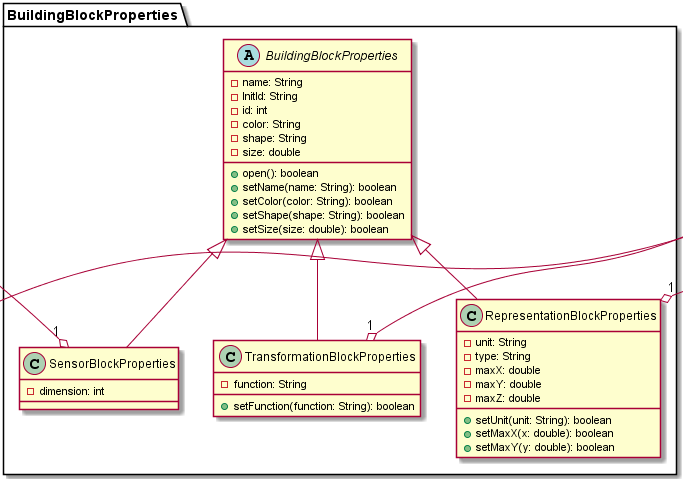
\includegraphics[width = 14cm]{Grafiken/View/BuildingBlockPropertiesNamespace.png}
		\caption{Aufbau des BuildingBlockProperties-Paket}
		\label{Entwurf_Grob}
	\end{center}
\end{figure}

Damit Benutzer Informationen über einzelne Bausteine bekommt, welche ihm das Benutzen der Anwendung erleichtern würden, wie auch eine tiefere Einsicht über die Funktionsweise bietet, stellt jeder Baustein ein eigenes "Eigenschaften-Menü" bereit, in welchem dem Benutzer die wichtigsten Eigenschaften zu sehen bekommt.

\clearpage

\begin{figure}[htbp]
	\begin{center}
		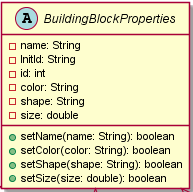
\includegraphics[width = 6cm]{Grafiken/View/BuildingBlockProperties.png}
		\caption{Aufbau der BuildingBlockProperties}
		\label{Entwurf_Grob}
	\end{center}
\end{figure}

\paragraph{BuildingBlockProperties}

Die abstrakte Klasse BuildingBlockProperties stellt alle Eigenschaften der konkreten Bausteine dar, welche alle Arten von Bausteinen (Sensor, Transformation, Darstellung) gemeinsam haben. Dazu gehören der Name,  Initialisierungs-ID, eindeutige Konfigurations-ID, Farbe, Form und Größe. Da einzelne Eigenschaften unveränderlich sein sollen, wie die IDs lassen sich nur Name, Farbe, Form und Größe verändern.

\paragraph{BuildingBlockPropertiesHandler}

\begin{figure}[htbp]
	\begin{center}
		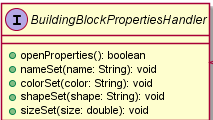
\includegraphics[width = 7cm]{Grafiken/View/BuildingBlockPropertiesHandler.png}
		\caption{Aufbau des BuildingBlockPropertiesHandler}
		\label{Entwurf_Grob}
	\end{center}
\end{figure}

Das Interface BuildingBlockPropertiesHandler wird von der Klasse BuildingBlockProperties implementiert und lässt den Benutzer durch mehrere Methoden das Eigenschaften-Fenster öffnen und Attribute der Baustein-Eigenschaften verändern. Bei allen Darstellungen von Konfigurationsbausteinen lässt sich der Name, Farbe, Form und Größe verändern.

\begin{figure}[htbp]
	\begin{center}
		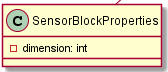
\includegraphics[width = 7cm]{Grafiken/View/SensorBlockProperties.png}
		\caption{Klasse SensorBlockProperties}
		\label{SensorBlockProperties}
	\end{center}
\end{figure}

\paragraph{SensorBlockProperties}

Neben den gemeinsamen Eigenschaften besitzt die Unterklasse SensorBlockProperties ebenfalls das Attribut der Dimension, welches darstellt über wie viele Kanäle dieser Sensor Messdaten liefert. Da dieses Attribut für Sensoren unveränderlich ist, kann diese ebenfalls vom Benutzer nicht verändert werden.

\begin{figure}[htbp]
	\begin{center}
		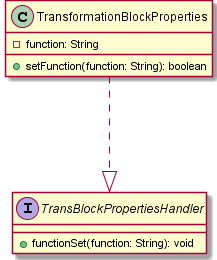
\includegraphics[width = 7cm]{Grafiken/View/TransformationBlockProperties.png}
		\caption{Aufbau der Klasse TransformationBlockProperties und dem Interface TransBlockPropertiesHandler}
		\label{Entwurf_Grob}
	\end{center}
\end{figure}

\paragraph{TransformationBlockProperties}

Transformationsbausteine besitzen neben den Standart-Eigenschaften noch eine vordefinierte Funktion für jeden Transformationsbaustein. Um dem Benutzer zu erlauben neue Transformationsbausteine zu definieren ist die Funktion veränderbar.

\paragraph{TransBlockPropertiesHandler}

Da der Benutzer bei einem Transformationsbaustein nur die Funktion verändern kann nimmt dieser Handler ebenfalls nur eine Benutzereingabe für eine Funktion entgegen und setzt diese in den Transformationsbaustein-Eigenschaften.

\begin{figure}[htbp]
	\begin{center}
		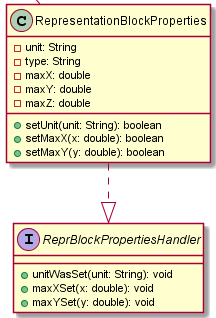
\includegraphics[width = 7cm]{Grafiken/View/RepresentationBlockProperties.png}
		\caption{Aufbau der Klasse RepresentationBlockProperties und Interface ReprBlockPropertiesHandler}
		\label{RepresentationBlockProperties}
	\end{center}
\end{figure}

\paragraph{RepresentationBlockProperties}

Da Repräsentatonsbausteine die visuelle Repräsentation beschreiben, besitzen diese für die Darstellung notwendige Eigenschaften, wie Einheit, Maximalwerte der Achsen und Art der Darstellung. Um den Benutzer die Möglichkeit zu geben die Darstellung auf die Messwerte anzupassen, lassen sich Einheit und Maximalwerte vom Benutzer einstellen, was über das Interface ReprBlockPropertiesHandler möglich ist.

\paragraph{ReprBlockPropertiesHandler}

Bei Repräsentationsbaustein-Eigenschaften ist der Benutzer in der Lage Einheit und Maximalwerte zu setzten. Daher nimmt der das Interface ReprBlockPropertiesHandler diese Benutzer eingaben entgegen und liefert diese weiter.


\newpage

\subsubsection{Button}

Knöpfe bieten dem Benutzer eine Anzahl von Funktion zur Bedienung der Anwendung an. Das Paket ButtonLayer enthält die konkreten Knöpfe, das Feld, in welchem die Knöpfe dargestellt werden und ein Interface für Benutzerinteraktionen.

\begin{figure}[htbp]
	\begin{center}
		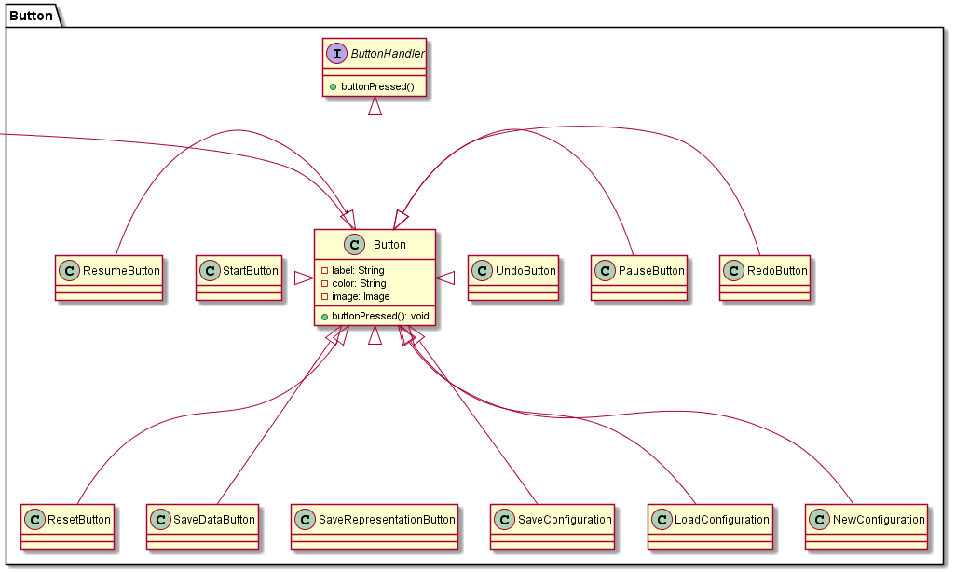
\includegraphics[width = 14cm]{Grafiken/View/ButtonNamespace.png}
		\caption{Aufbau des Button-Paket}
		\label{Entwurf_Grob}
	\end{center}
\end{figure}

\paragraph{Button}

Die Klasse Button ist die Überklasse zu den konkreten Knöpfen. Jeder Knopf enthält einen eindeutigen Namen und zur Unterscheidung der Knöpfe und zur einfachen Benutzung eine Farbe und ein aussagekräftiges Bild, welches die Funktionalität des Knopfes darstellt.

\paragraph{StartButton}

Die Klasse StartButton erbt von der Überklasse Button und stellt den Knopf dar, welcher bei Betätigung des Knopfes durch den Benutzer den Messlauf starten soll.

\paragraph{PauseButton}

Die Klasse PauseButton ist eine weitere Konkretisierung von Button und stellt den Knopf dar, welcher bei Betätigung durch den Benutzer einen Messlauf pausiert.

\paragraph{ResumeButton}

Die Klasse ResumeButton stellt den Knopf dar, welcher einen Messlauf fortsetzt, wenn der Benutzer diesen betätigt.

\paragraph{ResetButton}

Die Klasse ResetButton stellt den Knopf dar, welcher bei Betätigung durch den Benutzer den Messlauf auf den Ausgangszustand zurücksetzt.

\paragraph{SaveDataButton}

Die Klasse SaveDataButton stellt den Knopf dar, welcher dem Benutzer ermöglicht die Messwerte aus einem Messlauf zu speichern.

\paragraph{SaveRepresentationButton}

Die Klasse SaveRepresentationButton stellt den Knopf dar, welcher eine Momentaufnahme der graphischen Visualisierung der Messwerte speichern lässt.

\paragraph{SaveConfiguration}

Die Klasse SaveConfiguration stellt den Knopf dar, welcher dem Benutzer erlaubt seine eigene Messkonfiguration zu speichern.

\paragraph{LoadConfiguration} 

Die Klasse LoadConfiguration repräsentiert den Knopf, welcher eine gespeicherte Messkonfiguration in das Konfigurationsfeld laden lässt.

\paragraph{NewConfiguration}

Die Klasse NewConfiguration stellt den Knopf dar, welcher dem Benutzer die Funktion bietet eine neue Konfiguration zu erstellen.

\paragraph{UndoButton}

Die Klasse UndoButton stellt den Undo-Knopf dar, welcher bei Betätigung die letzte Benutzeraktion rückgängig macht.

\paragraph{RedoButton}

Die Klasse RedoButton stellt den Redo-Knopf dar, welcher die letzte rückgängig gemachte Aktion wiederherstellt.

\paragraph{Interface ButtonHandler}

Das Interface ButtonHandler registriert Benutzerinteraktionen auf der Benutzeroberfläche und löst die Methode ButtonPressed() aus, über welche die Anwendung die Benutzerinteraktion weiterverarbeitet.

\subsubsection{OptionAndHelp}

\begin{figure}[htbp]
	\begin{center}
		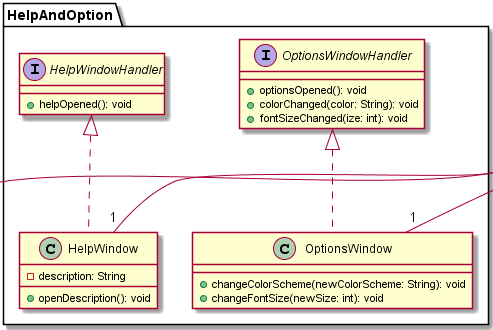
\includegraphics[width = 14cm]{Grafiken/View/HelpAndOptionNamespace.png}
		\caption{Aufbau des HelpAndOption-Paket}
		\label{Entwurf_Grob}
	\end{center}
\end{figure}

Das Paket OptionAndHelp soll dem Benutzer die Benutzung der Anwendung vereinfachen. Getrennt wurde das Paket in die Funktionsspezifische Klasse HelpWindow, welche dem Benutzer Hilfe zur Bedienung gibt und in die Klasse OptionsWindow, welche dem Benutzer Einstellungsmöglichkeiten gibt, um eine möglichst barrierefreie Benutzung zu ermöglichen.

\paragraph{HelpWindow}

Die Klasse HelpWindow beschreibt das Hilfe-Fenster der Anwendung. Der Benutzer bekommt bei Öffnen des Hilfe-Fensters eine allgemeine Erklärung zur Funktionalität und zur Bedienbarkeit der gesamten Anwendung. Ebenfalls könnte in dem Hilfstext ein einfaches Anwendungsbeispiel erklärt werden, um dem Benutzer erste Schritte zu vereinfachen.

\paragraph{OptionsWindow}

Die Klasse OptionsWindow stellt das Einstellungen-Fenster der Anwendung dar. Der Benutzer soll hierbei das verwendete Farbschema ändern können, um die Bedienung der Anwendung trotz möglichen Farbschwächen zu ermöglichen. Ebenfalls soll die Schriftgröße der Textelemente verändert werden können, um Sehschwächen auszugleichen und die Bedienbarkeit der Anwendung zu erhöhen. 

\paragraph{HelpWindowHandler}

Das Interface HelpWindowHandler, welches von der Klasse HelpWindow implementiert wird, liefert die Benutzereingabe im Falle des Drückens des Hilfe-Knopfes an die Anwendung weiter. Beim Drücken des Hilfe-Knopfes soll das Hilfefenster sofort erscheinen.

\paragraph{OptionsWindowHandler}

Das Interface OptionsWindowHandler, welches von der Klasse OptionsWindow implementiert wird, erkennt die Benutzereingabe im Falle des Drückens des "Einstellungen" oder "Optionen"- Knopf. In dem geöffneten Fenster kann der Benutzer dann das Farbschema und die Schriftgröße anpassen.

\newpage

\subsubsection{Exception}

\begin{figure}[htbp]
	\begin{center}
		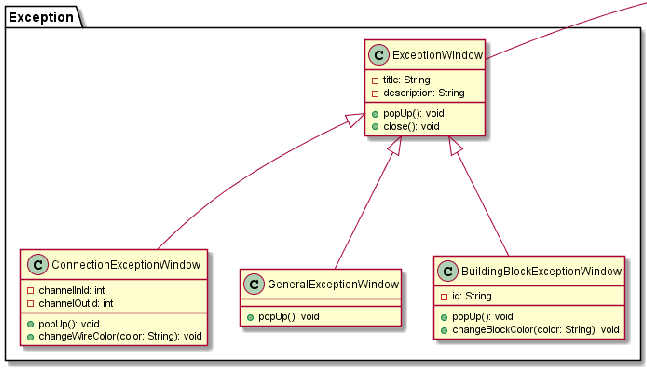
\includegraphics[width = 14cm]{Grafiken/View/ExceptionNamespace.png}
		\caption{Aufbau des Exception-Paket}
		\label{Entwurf_Grob}
	\end{center}
\end{figure}

Fehlernachrichten sind ein wichtiger Teil der Anwendung, um dem Benutzer eine möglichst benutzerfreundliche Umgebung zu liefern und eine möglichst einfache und verständliche Bedienung zu ermöglichen. Damit der Benutzer aussagekräftige Fehlermeldungen erhält unterscheiden wir im Entwurf zwischen drei Typen von Fehlerarten aus verschiedenen Fehlerquellen.

\paragraph{ExceptionWindow}

Die Klasse ExceptionWindow stellt die Überklasse der drei verschiedenen Unterklassen dar und enthält die gemeinsamen Attribute, welche die konkreten Fehlermeldungen enthalten. Eine Fehlermeldung besitzt immer eine Titel, der wünschenswerter Weise bereits die Fehlermeldung aussagekräftig und kurz beschreibt. Die Beschreibung der Fehlermeldung wiederum liefert eine genauere und explizite Erklärung zur Fehlerquelle, Fehlerursache und möglicherweise ebenfalls zur Fehlerbehebung.
Damit der Benutzer auf die Fehlernachricht aufmerksam wird, bewirkt die Methode popUp(), dass die Fehlernachricht zu sehen ist. Damit der Benutzer weiterarbeiten kann oder den Fehler beheben will kann die Fehlernachricht wieder geschlossen werden.

\paragraph{BuildingBlockExceptionWindow}

Die Klasse BuildingBlockExceptionWindow ist eine Konkretisierung der Überklasse ExceptionWindow und stellt eine Fehlernachricht im Bezug zu Konfigurationsbausteinen dar. Neben einem Titel und einer Beschreibung wird zur Erzeugung dieser Fehlernachricht die eindeutige ID des Konfigurationsbausteins benötigt. Dadurch erfährt der Benutzer sofort, bei welchem Konfigurationsbaustein ein Fehler aufgetreten ist. Die Methode popUp() aus der Überklasse wird hier überschrieben. Damit soll bewirkt werden, dass die Fehlermeldung als Pop-Up Nachricht direkt neben dem Konfigurationsbaustein im Konfigurationsfeld erscheint und somit dem Benutzer sofort die Fehlerquelle signalisiert. Ebenfalls wird zur Darstellung des Fehlers die Farbe des Konfigurationsbaustein im Konfigurationsfeld geändert, um dem Benutzer nochmal auf die Fehlerquelle hinzuweisen.

\paragraph{ConnectionExceptionWindow}

Die Klasse ConnectionExceptionWindow ist eine weitere Konkretisierung der Überklasse ExceptionWindow und stellt eine Fehlernachricht bei Verbindungen zwischen Konfigurationsbausteinen dar. Zur Identifizierung der Fehlerquelle wird neben Titel und Beschreibung ebenfalls die IDs der Ein- und Ausgangskanäle der Konfigurationsbaustein mit übergeben. Die Methode popUp() soll ebenfalls die Fehlernachricht in der Nähe der Fehlerquelle im Konfigurationsfeld plazieren. Ebenfalls wird die Farbe des Drahtes sinnvoll verändert um die Fehlerquelle zu signalisieren.

\paragraph{GeneralExceptionWindow}

Die Klasse GeneralExceptionWindow stellt neben den zwei konkreten Fehlermeldungen ConnectionExceptionWindow und BuildingBlockExceptionWindow eine allgemeinere Fehlernachricht dar. Diese werden zum Beispiel bei Messfehlern oder Fehler bei der Messkonfiguration ausgelöst. Diese Fehlernachrichten sollen sichtbar in der Mitte der Anwedung geöffnet werden, um dem Benutzer auf diesen Fehler hinzuweisen. 

\paragraph{ExceptionWindowManager}

Die Klasse ExceptionWindowManager nimmt Fehlermeldungen entgegen und stößt die Visualisierung der jeweilig nach Fehlermeldung unterschiedlichen Fenster an. Der Klasse werden die für eine Fehlermeldung notwendigen Parameter Titel und  Beschreibung übergeben. Je nach Art der Fehlermeldung wird auch die Baustein- oder Verbindung-ID der Fehlerquelle übergeben.

\subsubsection {FacadeModelView}

\begin{figure}[htbp]
	\begin{center}
		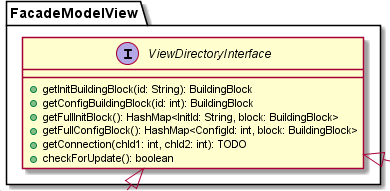
\includegraphics[width = 12 cm]{Grafiken/View/FacadeModelViewNamespace.png}
		\caption{Aufbau des FacadeModelView-Paket}
		\label{Entwurf_Grob}
	\end{center}
\end{figure}

Das Paket FacadeModelView enthält das Interface, welches das Model anbietet und vom View verwendet wird. Da durch das Directory eine Art Zwischenschicht zwischen Model und View darstellt wird ersetzt die Fassade zum Directory eine unübersichtliche Fassade zu dem Model. 

\paragraph{ViewDirectoryInterface}

Das Interface ViewDirectoryInterface bietet wichtige Funktionen an, um Änderungen am Model in die GUI zu übertragen. 
Bei dem Starten der Anwendung werden alle über das Backend übertragenen Bausteine durch das Model in das Directory geladen. Um alle Bausteine in die GUI zu laden gibt die Methode getFullInitBlock() die gesamte Hash-Map, welche die Konfigurationsbausteinen enthält zurück um daraus die Prototypenmenüs zu erstellen. Um einzelne Bausteine mit bestmmter aus dem Directory zu laden gibt es die Methoden getInitBuildingBlock() und getConfigBuildingBlock(). Um eine gespeicherte Verbindung zu bekommen gibt es die Methode getConnection(chId1: int, chId2: int), welche zwei ChannelDecorater-IDs mit übergibt und die Verbindung zurückgibt.
Damit das View bei Benachrichtigung über ein Update des Models überprüfen kann, ob das Directory Änderungen enthält gibt es die Methode checkForUpdates(), welche einen Wahrheitswert zurückgibt, welcher eine Aussage über die Änderungen am Directory enthält.

\clearpage

\subsubsection{FacadeControllerView}

\begin{figure}[htbp]
	\begin{center}
		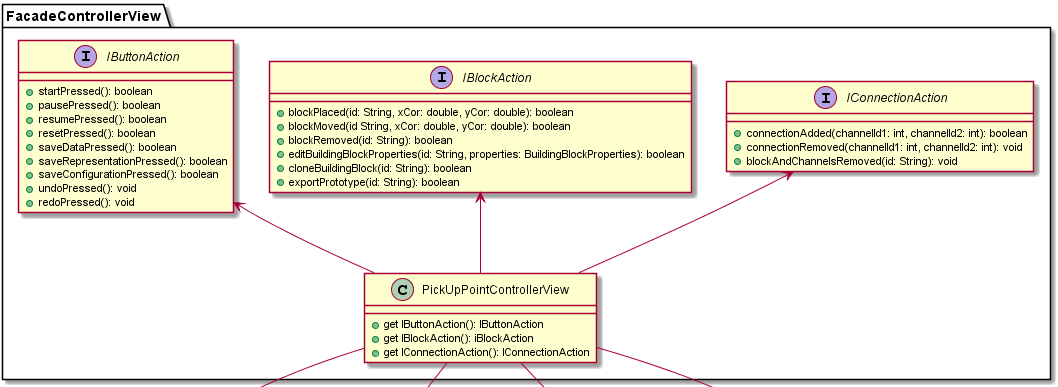
\includegraphics[width = 14 cm]{Grafiken/View/FacadeControllerViewNamespace.png}
		\caption{Aufbau des FacadeControllerView-Paket}
		\label{Entwurf_Grob}
	\end{center}
\end{figure}

Das Paket FacadeControllerView stellt die Schnittstelle dar, welche der Controller anbietet und vom View benutzt wird. Zur Übersicht ist die Fassade intern in 3 Interfaces aufgeteilt, welche jeweils Funktionen eines Objektes darstellen (Button, Block, Connection). Eine PickUp-Klasse stellt die Anbindung zum View dar und kapselt die Interfaces.

\begin{figure}[htbp]
	\begin{center}
		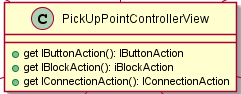
\includegraphics[width = 8 cm]{Grafiken/View/PickUpPoint.png}
		\caption{Die Klasse PickUpPointControllerView}
		\label{PickUpPointControllerView}
	\end{center}
\end{figure}

\paragraph{PickUpPointControllerView}

Die Klasse PickUpPointControllerView stellt die Schnittstelle zwischen den Interfaces und den Klassen, welche auf diese zugreifen dar. Ihre Methoden liefern jeweils das gewollte Interface zurück, über welches dann Aktionen an den Controller übergeben werden können.

\clearpage

\begin{figure}[htbp]
	\begin{center}
		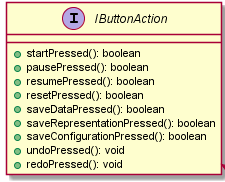
\includegraphics[width = 7 cm]{Grafiken/View/IButtonAction.png}
		\caption{Das Interface IButtonAction}
		\label{Entwurf_Grob}
	\end{center}
\end{figure}

\paragraph{IButtonAction}

Das Interface IButtonAction liefert eine Schnittstelle für alle Knopf-Aktionen. Dass heißt, wenn durch den ButtonHandler eine Benutzereingabe in Form des Drücken eines konkreten Knopfes registriert wird, wird in diesem Interface die für den Knopf spezifische Methode aufgerufen, um den Controller zu benachrichtigen. Dabei gibt es für jeden konkreten Knopf eine Interface-methode.

\begin{figure}[htbp]
	\begin{center}
		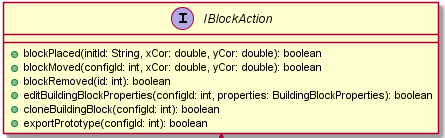
\includegraphics[width = 10 cm]{Grafiken/View/IBlockAction.png}
		\caption{Das Interface IBlockAction}
		\label{IBlockAction}
	\end{center}
\end{figure}

\paragraph{IBlockAction}

Das Interface IBlockAction liefert eine Schnittstelle für alle Benutzerinteraktionen mit einem Konfigurationsbaustein. Diese gibt das Interface weiter an den Controller, in dem das Interface implementiert ist. Die Methode blockPlaced gibt hierbei weiter, wenn ein Konfigurationsbaustein aus einem dem Prototypen Menüs auf das Konfigurationsfeld per Drag-and-Drap platziert wurde. Hierbei wird die Prototyp-spezifische ID mitgegeben und die Koordinaten, welche die Position des Bausteins eindeutig bestimmen. Die Methode blockMoved wird dann benutzt, wenn ein Konfigurationsbaustein innerhalb des Konfigurationsfeldes die Position ändert. Wenn der Benutzer einen Konfigurationsbaustein aus dem Konfiguratonsfeld entfernt wird dies über die Methode blockRemoved mit Übergabe der eindeutigen ID an den Controller überliefert. Wenn der Benutzer die Eigenschaften eines Bausteinprototyps ändert wird dies über die Methode editBuildingBlockProperties mit der eindeutigen ID und den neuen Eigenschaften übergeben. Wenn ein Baustein geklont oder exportiert werden soll, wird dies mit der Übergabe der eindeutigen ID an den Controller übergeben.

\begin{figure}[htbp]
	\begin{center}
		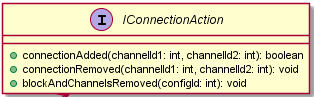
\includegraphics[width = 9 cm]{Grafiken/View/IConnectionAction.png}
		\caption{Das Interface IConnectionAction}
		\label{IConnectionAction}
	\end{center}
\end{figure}

\paragraph{IConnectionAction}

Das Interface IConnectionAction liefert eine Schnittstelle für Aktionen, welche der Benutzer mit Verbindungen macht. 
Die Methode connectionAdded übergibt dem Controller zwei eindeutige Channel-IDs, welche der Benutzer miteinander verbunden hat, um eine Messkonfiguration aufzubauen.
Wenn der Benutzer eine Verbindung zwischen zwei Konfigurationsbausteinen entfernt übergibt die Methode connectionRemoved die zwei Channel-IDs an den Controller um diese Verbindung aus der Messkonfiguration zu entfernen.
Falls der Benutzer einen Konfigurationsbaustein entfernt, welcher bereits mit weiteren Konfigurationsbausteinen verbunden war, werden diese Verbindungen ebenfalls gelöscht, daher wird bei der Methode blockAndChannelsRemoved nur die eindeutige Konfigurationsblock-ID übergeben.

\clearpage
\section{Sequenzdiagramme}



\subsection{Block hinzufügen komplett}

\begin{figure}[htbp]
	\begin{center}
		\includegraphics[width = 16cm]{Grafiken/SeqAddBPart1.png}
		\caption{Das Hinzufügen eines Bausteins zur Messkonfiguration und dessen Darstellung in der GUI, Part1}
		\label{SeqAddBPart1}
	\end{center}
\end{figure}

\begin{figure}[htbp]
	\begin{center}
		\includegraphics[width = 16cm]{Grafiken/SeqAddBPart2.png}
		\caption{Das Hinzufügen eines Bausteins zur Messkonfiguration und dessen Darstellung in der GUI.}
		\label{SeqAddBPart2}
	\end{center}
\end{figure}



In den Abbildungen \ref{SeqAddBPart1} und \ref{SeqAddBPart2} ist das Szenario "`Block hinzufügen komplett zu sehen"'. Als Ausgangspunkt registriert der DragAndDropHandler der GUI, dass ein Block an die entsprechende Stelle im Konfigurationsfeld platziert wurde. Die GUI benachrichtigt den Controller über das Interface BlockAction, dass ein Block platziert wurde. Der Controller erstellt einen entsprechenden Command und lässt die Änderung am Model durchführen. Dazu greift er über die Schnittstelle IModelInformation auf die Messkonfiguration im Model zu, um einen Block hinzu zufügen. Die Messkonfiguration im Model führt einige Methoden aus, um sich eine Kopie des angeforderten Bausteinprototyps von dem BuildingBlockDirectory zu holen. Außerdem wird dem Block eine ConfigId beigefügt. Danach wird er der ConfigHashMap des BuildingBlockDirectory hinzugefügt. Dann wird dem Konfigurationsfeld GUI über die Schnittstelle UpdateInterface signalisiert, dass die Messkonfiguration verändert wurde. Dieses prüft nach, was sich im BuildingBlockDirectory verändert hat und holt sich dann das Update. Sobald das Update im Konfigurationsfeld der GUI angekommen ist, wird das Feld mit dem entsprechenden BlockView geupdatet.

\subsection{Block hinzufügen, undo, redo}

\begin{figure}[htbp]
	\begin{center}
		\includegraphics[width = 16cm]{Grafiken/AddBlockSequence.png}
		\caption{Das Hinzufügen eines Bausteins zur Messkonfiguration, außerdem das rückgängig machen und wiederherstellen dieser Aktion.}
		\label{AddBlockSequence}
	\end{center}
\end{figure}

In Abbildung \ref{AddBlockSequence} ist das Szenario "AddBlockSequence" zu sehen. Dabei wird hier vor allem auf den undo und redo Aspekt eingegangen. Der Ablauf des oberen Teils ähnelt stark dem Ablauf des vorherigen Sequenzdiagramms und wird nicht noch mal wiederholt. Im zweiten Teil wird als Ausgangspunkt der UnDo-Knopf in der GUI gedrückt. Dadurch wird der CommandManager Controller über das Interface ButtonAction angeleitet, den UnDo-Command durchzuführen. Dieser führt den Befehl durch und entfernt den Block wieder aus dem Model.

Im dritten Teil soll die UnDo-Action des zweiten Teiles rückgängig gemacht werden. Dazu wird als Ausgangspunkt der ReDo-Knopf in der GUI gedrückt. Dadurch wird der CommandManager Controller über das Interface ButtonAction angeleitet, den ReDo-Command durchzuführen. Dieser führt den Befehl durch und fügt den Block wieder dem Model hinzu.


\clearpage
\section{Änderungen am Pflichtenheft}

Durch unsere Entscheidungen im Entwurfsdokument bekommt der Benutzer Hilfe für die Verwendung der Anwendung und soll durch Informationen und Hilfestellungen zu einzelnen Bausteinen in der Lage sein eine korrekte Messkonfiguration aufzubauen.
Falls der Benutzer trotzdem eine nicht verwendbare Messkonfiguration aufbaut, wird er bei Starten der Messung durch eine Fehlermeldung darauf hingewiesen.
Daraus folgt, dass Soll-Kriterium 13 aus dem Pflichtenheft nicht vollständig erfüllt ist, da die Anwendung keine Warnungen vor falschen Benutzereingaben vorsieht, sondern nur reaktionär Fehlermeldungen auf Fehlverhalten ausgibt.

Ebenfalls haben wir uns entschieden, um eine zu starke Belastung der Teammitglieder während der Implementierung und eine falsche Prioritätensetzung zu vermeiden Wunschkriterien, welche nicht für die Funktionalität der Anwendung und zur einfacheren Implementieren beitragen nicht in den Entwurf miteinzubeziehen. 
Dazu gehören das Wunschkriterium Wunsch-Kriterium 3, welches Spiele zum Erlernen von grundlegenden Messtechniken vorsah. Da der Entwurf dieses Feature, wie auch die Implementierung in unserer Software sehr Zeit intensiv wäre. Für zukünftige Weiterentwicklung der Anwendung wäre so ein Feature jedoch sehr interessant und sollte deswegen nicht verworfen werden.
Ebenfalls haben wir Wunsch-Kriterium 5, welches die Funktion darstellt eine Darstellung von visualisierten Messdaten auszudrucken nicht direkt in die Anwendung implementiert. 
Wunsch-Kriterium 6 wurde ebenfalls nicht in den Entwurf miteinbezogen, jedoch wäre, je nach verwendeter Software zur Implementierung der graphischen Benutzeroberfläche eine solche Änderung der Sprache möglich, jedoch haben wir uns aus zeitlichen und organisatorischen Gründen dagegen entschieden, den Mehraufwand dafür in Kauf zu nehmen.


\clearpage
\section{Anhang}


\clearpage
\subsection{Vollständiges Klassendiagramm}


\clearpage
\section{Glossar}\label{glossar}

\renewcommand*{\glossarysection}[2][]{}	% prevents double glossary section heading
\printnoidxglossaries				% generate pdf twice when adding new entries


\end{document}\grid
